\documentclass[aspectratio=169]{beamer}
\usepackage{animate}
\usepackage{tikz}
\usetheme{metropolis}

% Bibliography setup
\usepackage{natbib}
\bibliographystyle{apalike}

\title{Bayesian anomaly detection for Cosmology - 21cm, Supernovae, and beyond}
\subtitle{Sam Leeney}
\date{May 27, 2025}
\author{With: Will Handley, Eloy de Lera Acedo, Harry Bevins}
\institute{} % Can be filled in later if needed
\setbeamertemplate{footline}{
\leavevmode%
\hbox{%
\begin{beamercolorbox}[wd=.33\paperwidth,ht=2.5ex,dp=1ex,leftskip=3mm]{author in head/foot}%
\tiny Sam Leeney
\end{beamercolorbox}%
\begin{beamercolorbox}[wd=.33\paperwidth,ht=2.5ex,dp=1ex,center]{title in head/foot}%
\tiny sakl2@cam.ac.uk
\end{beamercolorbox}%
\begin{beamercolorbox}[wd=.33\paperwidth,ht=2.5ex,dp=1ex,rightskip=3mm]{date in head/foot}%
\tiny \href{https://github.com/samleeney}{github.com/samleeney/Talks}
\end{beamercolorbox}%
}%
\vskip0pt%
}


\begin{document}

\begin{frame}
  \titlepage
\end{frame}

\begin{frame}{Outline}
  \tableofcontents[hideallsubsections]
\end{frame}


\section{Bayesian anomaly detection}

\begin{frame}{Over simplified example of anomaly detection method (thresholding)}
  \footnotesize
  \textbf{Simple statistical approach:}
  \begin{itemize}
    \item Calculate mean ($\mu$) and standard deviation ($\sigma$) of the data
    \item Define threshold $T = \mu + k\sigma$ where $k$ is a sensitivity parameter
    \item Flag data point $x_i$ as anomalous if:
  \end{itemize}
  \begin{equation}
    \text{anomaly}_i = \begin{cases}
      1 & \text{if } x_i > T \\
      0 & \text{otherwise}
    \end{cases}
  \end{equation}
  \textbf{Limitations:}
  \begin{itemize}
    \item Choice of $k$ is arbitrary
    \item Assumes Gaussian statistics
    \item No consideration of temporal correlations
    \item Cannot distinguish between RFI and real signals
  \end{itemize}
\end{frame}

\begin{frame}{Thresholding results}
  \begin{columns}
    \column{0.5\textwidth}
    \textbf{Constant signal with RFI:}
    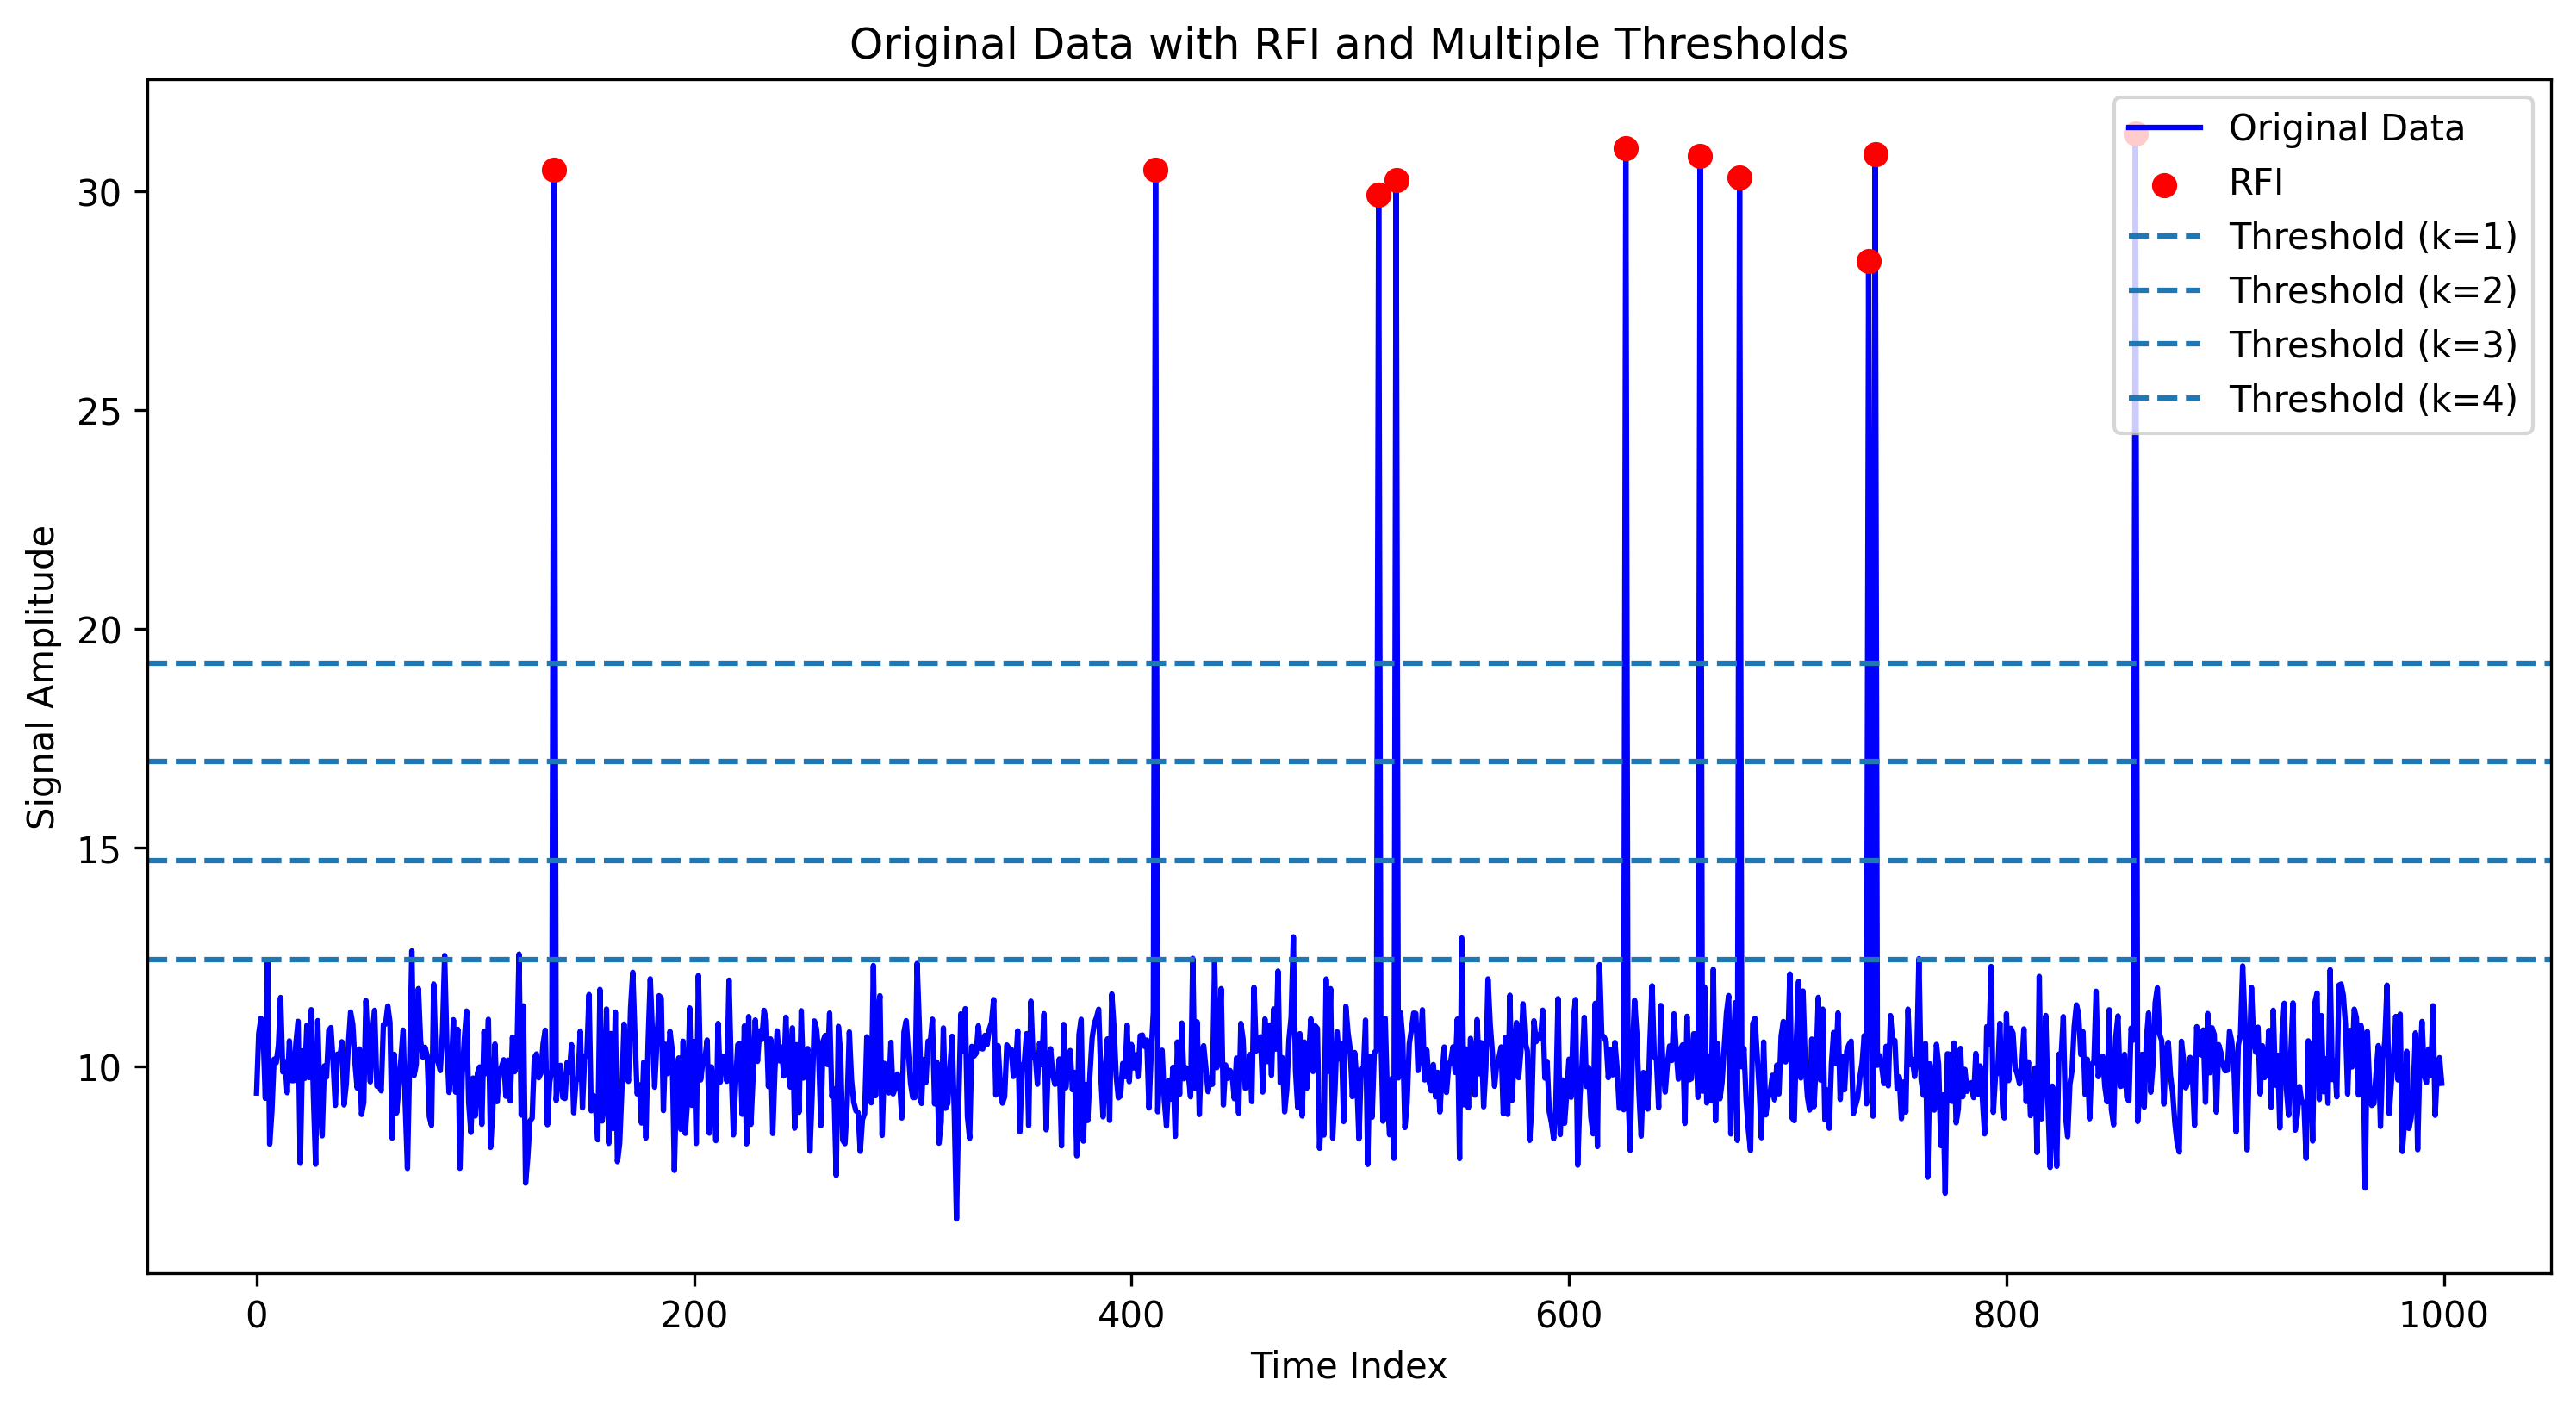
\includegraphics[width=1\textwidth]{images/threshold_multiple.png}
    \column{0.5\textwidth}
    \textbf{Sine wave with RFI:}
    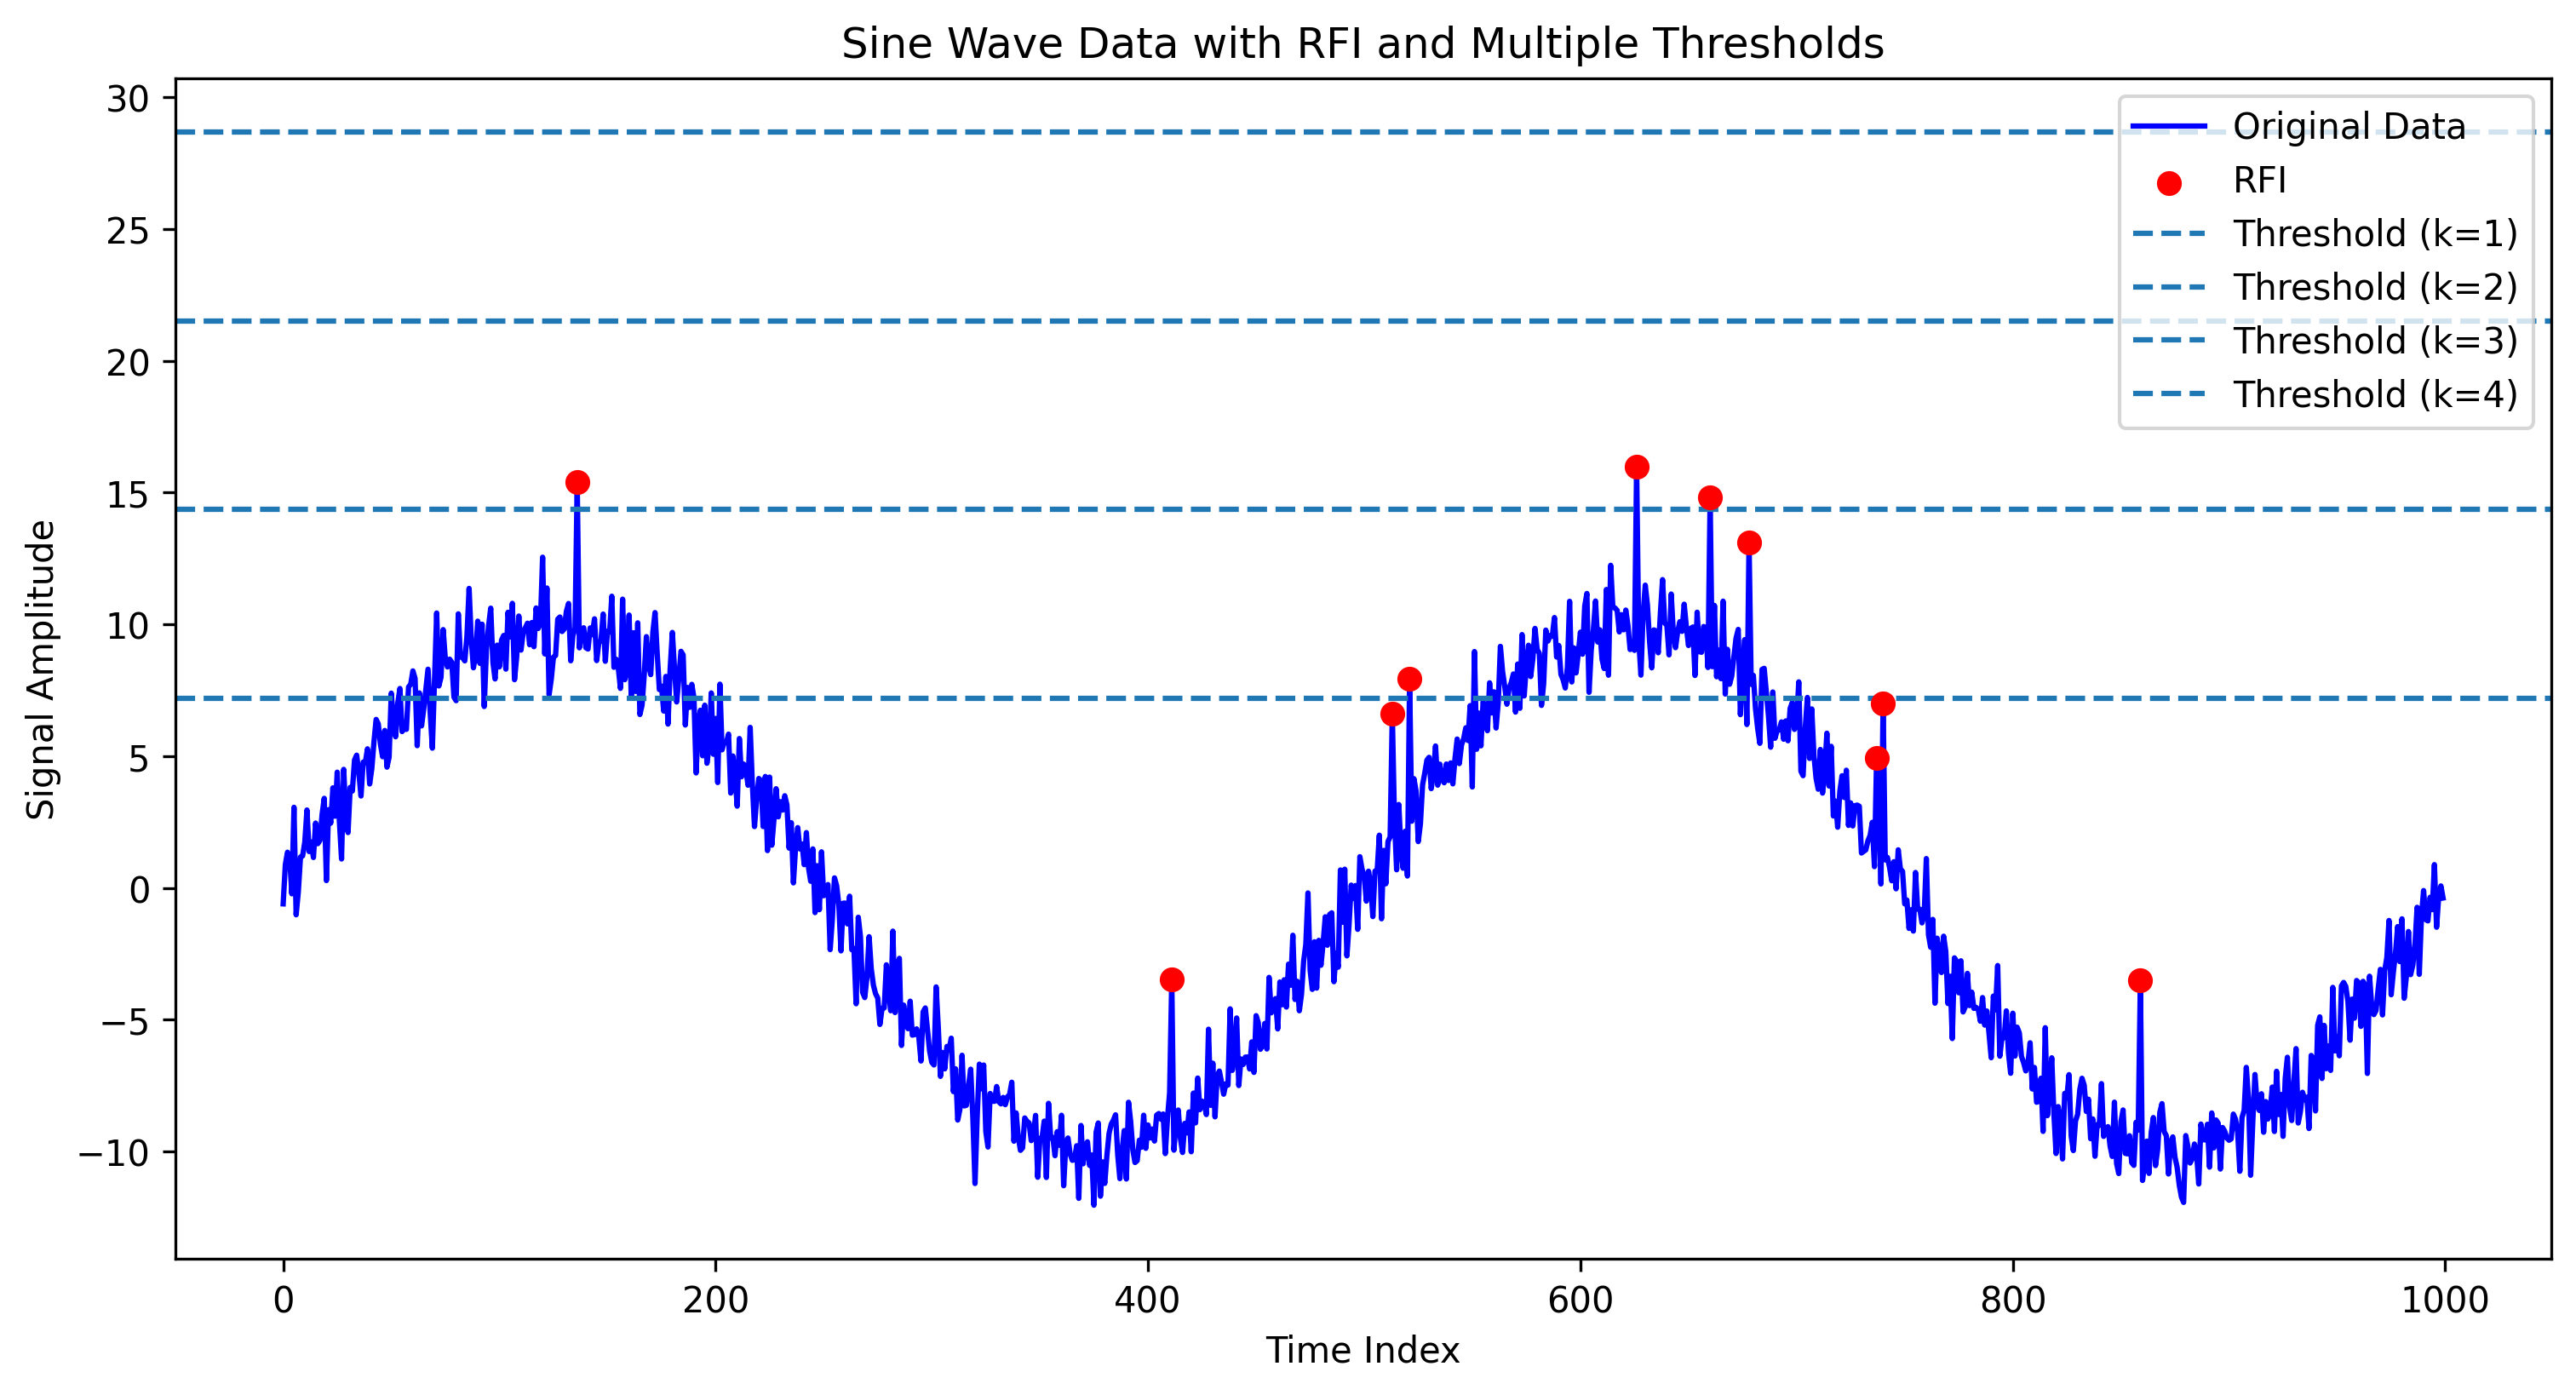
\includegraphics[width=1\textwidth]{images/threshold_sin_multiple.png}
  \end{columns}
  \begin{itemize}
    \item Traditional methods are generally not model aware.
    \item Anomalies are typically sought either before or after typical fitting process.
  \end{itemize}
\end{frame}

\begin{frame}{Model anomalies in via a method that is:}
  \begin{itemize}
    \item Model aware
    \item Works simultaneously with model fitting
    \item Not binary, ie encodes 'belief' datum are anomalous
  \end{itemize}
\end{frame}

\begin{frame}{Define anomaly mask $\varepsilon$}
  \begin{columns}
    \column{0.25\textwidth} % Equation on the left, 25% width
      \footnotesize
      \begin{equation}
          \varepsilon_i = \begin{cases}
              0 &: \text{expected}\\
              1 &: \text{anomalous},
          \end{cases}
      \end{equation}
    \column{0.75\textwidth} % Image on the right, 75% width
      \centering
      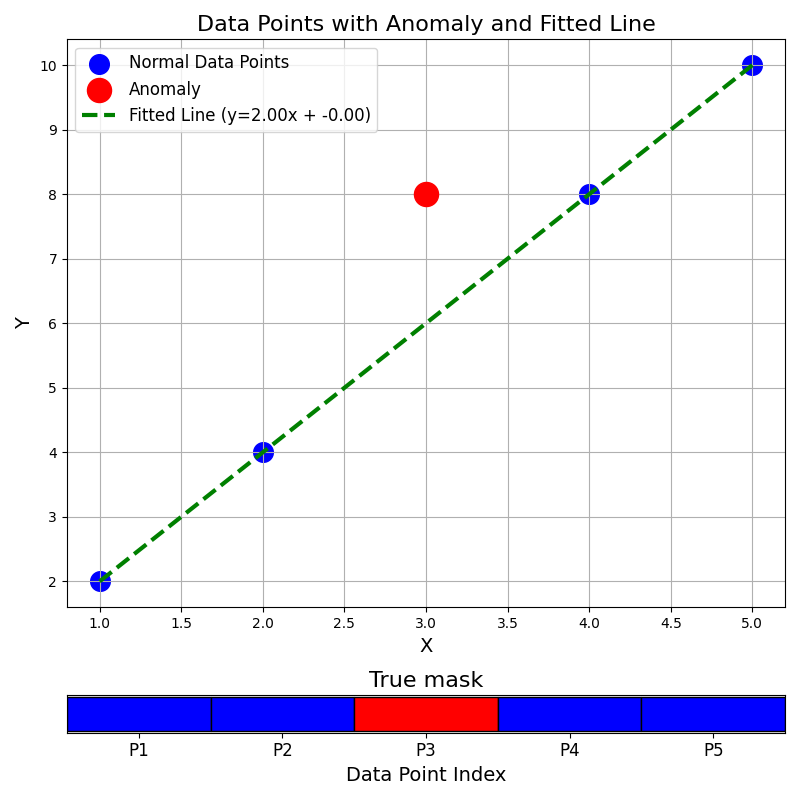
\includegraphics[width=0.7\textwidth]{images/generated_plot.png} % Image should fill its column
  \end{columns}
\end{frame}

\begin{frame}{Ascribe Bernoulli prior to $\varepsilon$}
  \footnotesize
  \begin{equation}
      P(\varepsilon_i) = p^{\varepsilon_i}(1-p)^{(1-\varepsilon_i)}.
  \end{equation}
  \begin{itemize}
    \item A Bernoulli prior assigns a probability $p$ to a binary variable being 1 (anomalous) and $1-p$ to it being 0 (expected).
  \end{itemize}
\end{frame}


\begin{frame}{Peicewise likelihood with $\varepsilon$}
    \centering
    The likelihood function before marginalizing over $\epsilon$ is given by:
    $$P(\vec{D}, \vec{\epsilon} | \theta) = \prod_{i=1}^{N} \left(L_i(\theta) (1-p)\right)^{(1-\epsilon_i)} \left(\frac{p}{\Delta}\right)^{\epsilon_i}$$
    Where:
    \begin{itemize}
        \item $L_i(\theta)$ is the likelihood of the $i$'th data point $D_i$ under the "expected" model.
        \item $\Delta$ is a constant related to the "anomalous" model.
        \item $p$ is the prior probability that a data point is anomalous ($P(\epsilon_i = 1)$).
        \item $\epsilon_i$ is a binary variable: $\epsilon_i = 0$ for expected, $\epsilon_i = 1$ for anomalous.
    \end{itemize}
\end{frame}

\begin{frame}{Marginalise over epsilon}
  \footnotesize
  \begin{equation}
      P(\mathcal{D} | \theta) =\sum_{\varepsilon \in \{ 0, 1 \} ^N}P(\mathcal{D},\varepsilon|\theta)
  \end{equation}
  \begin{center}
    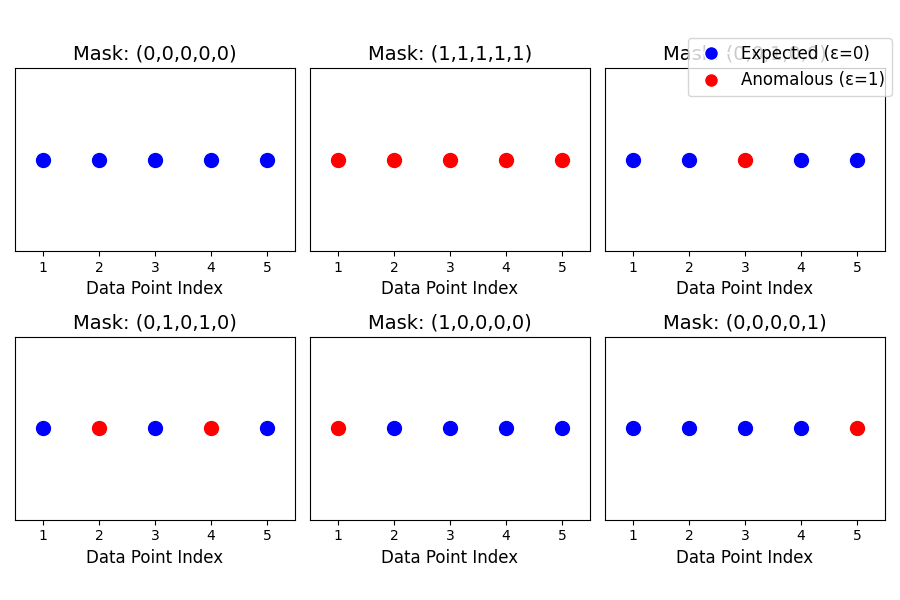
\includegraphics[width=0.64\textwidth]{images/marginalize_epsilon_plot.png}
  \end{center}
\end{frame}
\begin{frame}{Likelihood After Marginalization}
    \centering
    The likelihood function after marginalizing over $\epsilon$ is given by:
    $$L(D | \theta) = \prod_{i=1}^{N} \left( (1-p) L_i(\theta) + p \frac{1}{\Delta} \right)$$
    Where:
    \begin{itemize}
        \item $D = \{D_1, D_2, \dots, D_N\}$ represents the dataset of $N$ data points.
        \item $\theta$ represents the model parameters.
        \item $L_i(\theta)$ is the likelihood of the $i$-th data point $D_i$ being "expected".
        \item $p$ is the prior probability that a single data point is "anomalous".
        \item This is computationally impractical as mask scales $2^N$.
    \end{itemize}
\end{frame}

\begin{frame}{Approximate correct mask is most likely}
  \footnotesize
  \begin{equation}
      P(\mathcal{D}|\theta, \varepsilon_{\mathrm{max}}) \gg \mathrm{max}_j P(\mathcal{D}|\theta,\varepsilon^{(j)})\label{eq:nlo},
  \end{equation}
  \begin{center}
    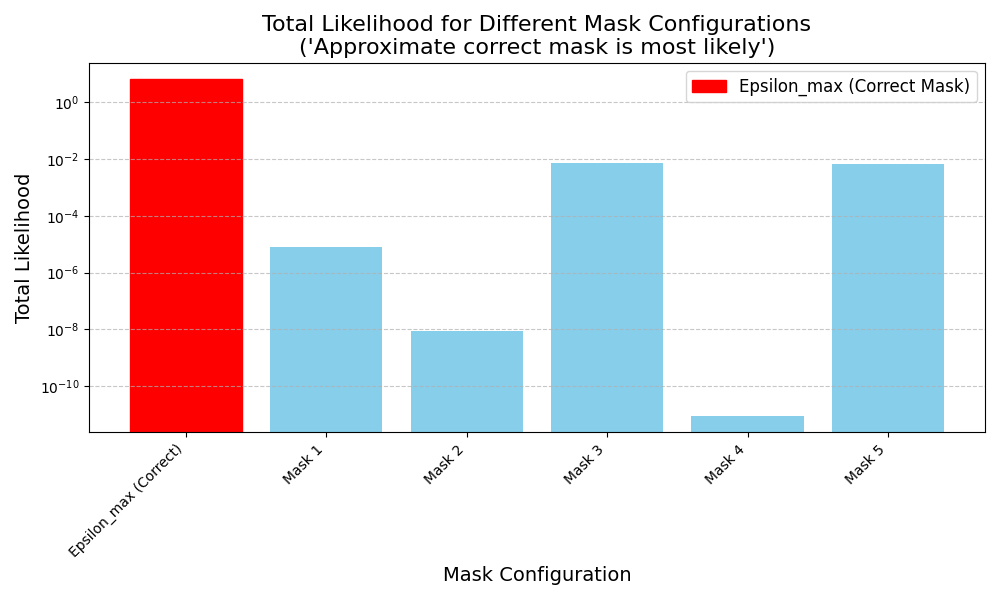
\includegraphics[width=0.64\textwidth]{images/dominant_mask_plot.png}
  \end{center}
\end{frame}

\begin{frame}{Loglikelihood and Maximisation}
  \footnotesize
  \textbf{e) Loglikelihood:}
  \begin{equation}
      \log{P(\mathcal{D}|\theta)} = \sum_{i}[{\log{\mathcal{L}_i}+\log({1-p})]\varepsilon^{\mathrm{max}}_i + [\log{p} - \log{\Delta}](1 - \varepsilon^\mathrm{max}_i})
  \end{equation}

  \textbf{f) Find the mask that $\varepsilon^{max}$ that maximises the likelihood by comparing the terms:}
  \begin{equation}
  \log P(\mathcal{D}|\theta) =
  \begin{cases}
  \log \mathcal{L}_i + \log(1 - p), & \text{if } [\log \mathcal{L}_i + \log(1 - p) > \log p - \log \Delta] \\
  \log p - \log \Delta, & \text{otherwise}
  \end{cases}
  \end{equation}
\end{frame}

\begin{frame}{Fit on a simple toy model}
    \centering
    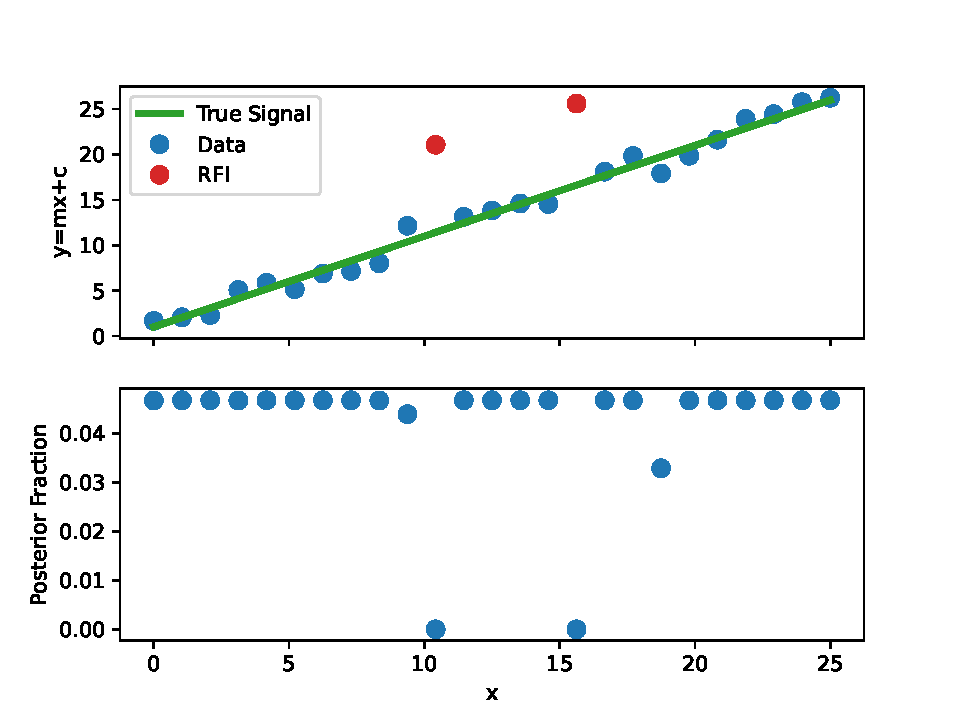
\includegraphics[width=0.56\textwidth]{images/test.pdf}
\end{frame}

\begin{frame}{We are imposing a 'floor' on our likelihood}
    \begin{columns}
        \column{0.5\textwidth}
            \centering
            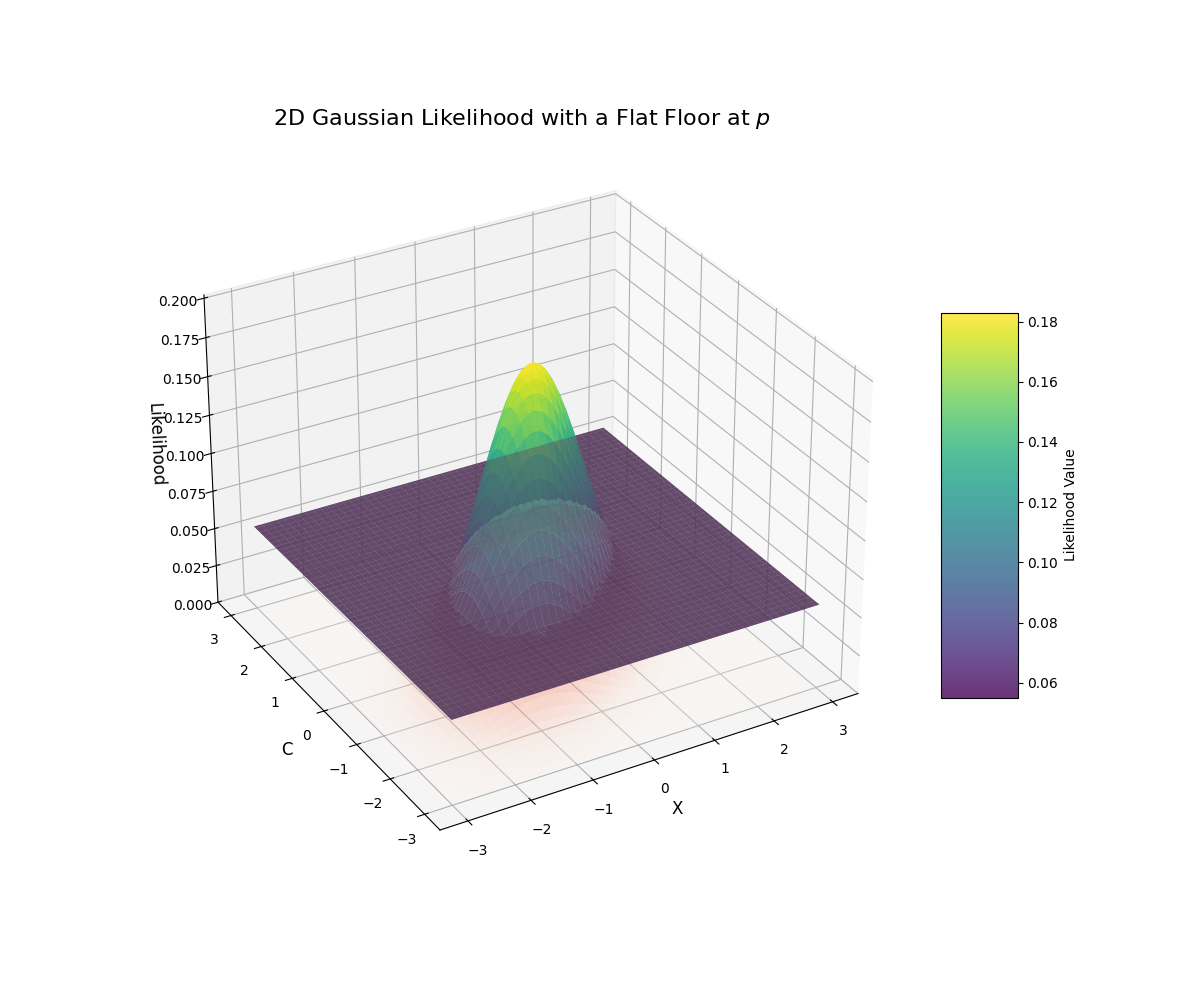
\includegraphics[width=1.2\textwidth]{images/likelihood_floor_plot.png}
        \column{0.5\textwidth}
            \centering
            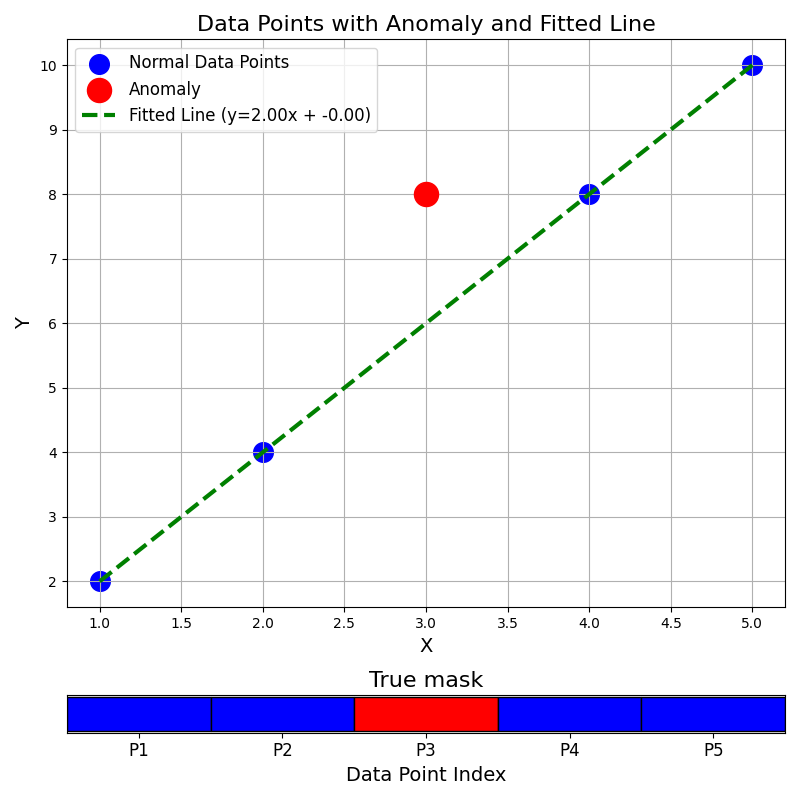
\includegraphics[width=0.7\textwidth]{images/generated_plot.png}
    \end{columns}
\end{frame}

\begin{frame}{Varying $p$}
    \centering
    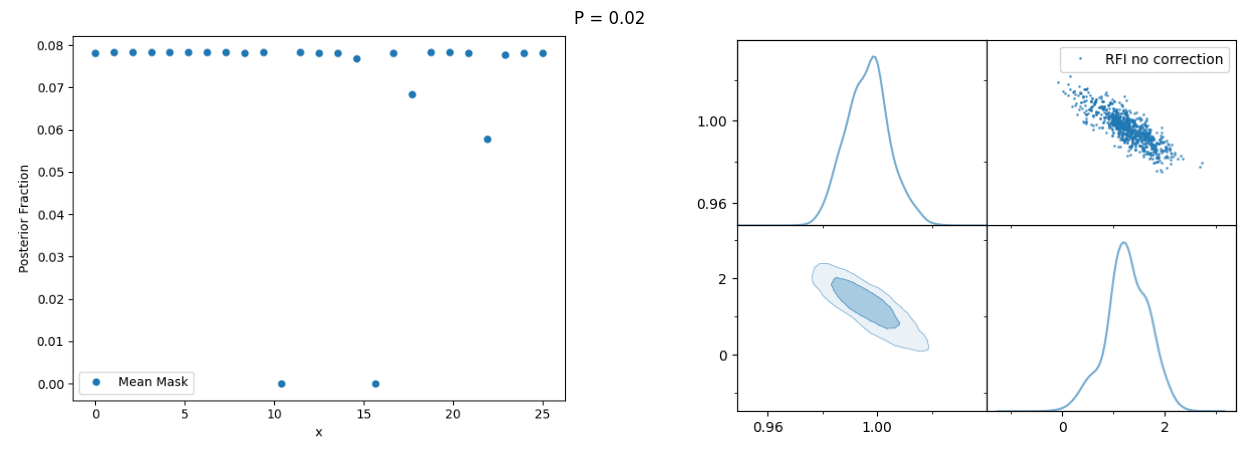
\includegraphics[width=0.8\textwidth]{images/gif_anest/comb_2.png}
\end{frame}

\begin{frame}{Varying $p$}
    \centering
    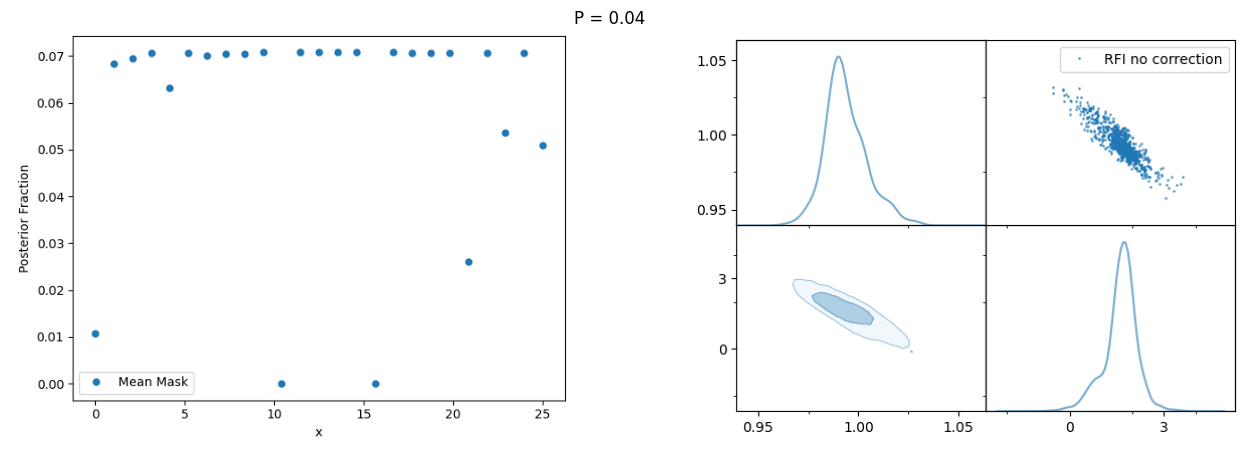
\includegraphics[width=0.8\textwidth]{images/gif_anest/comb_3.png}
\end{frame}


\begin{frame}{Varying $p$}
    \centering
    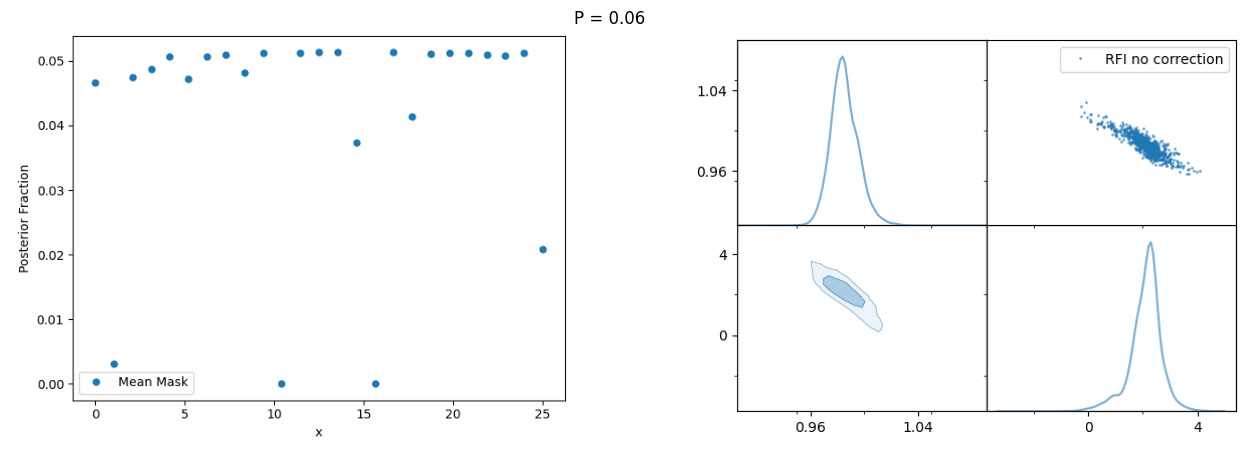
\includegraphics[width=0.8\textwidth]{images/gif_anest/comb_4.png}
\end{frame}

\begin{frame}{Varying $p$}
    \centering
    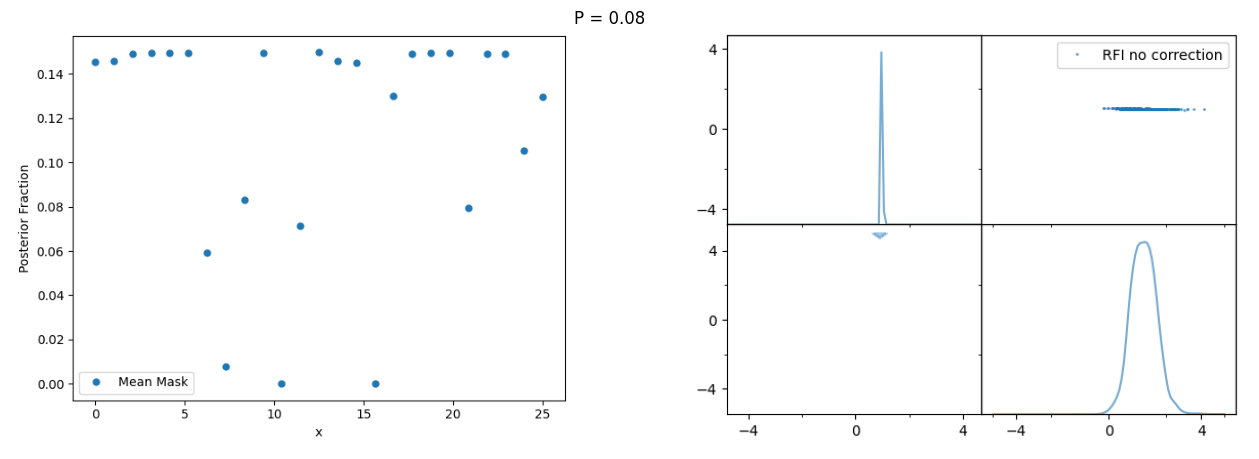
\includegraphics[width=0.8\textwidth]{images/gif_anest/comb_5.png}
\end{frame}

\begin{frame}{Varying $p$}
    \centering
    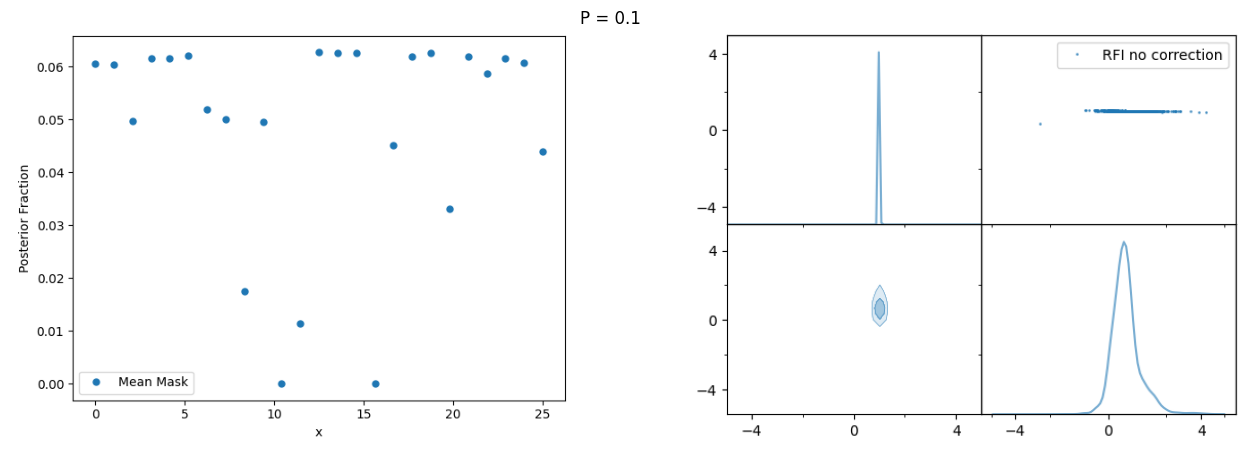
\includegraphics[width=0.8\textwidth]{images/gif_anest/comb_6.png}
\end{frame}

\begin{frame}{Varying $p$}
    \centering
    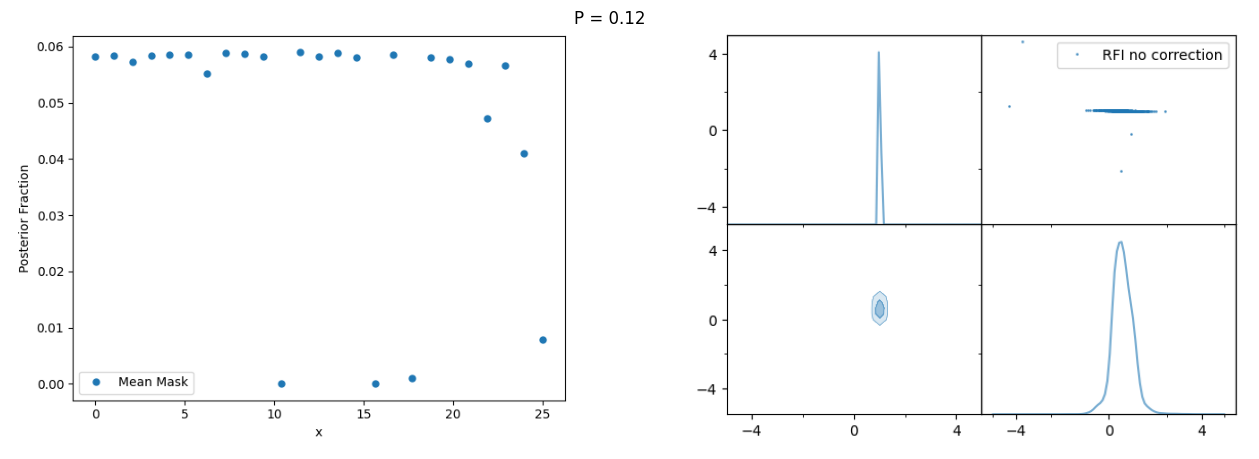
\includegraphics[width=0.8\textwidth]{images/gif_anest/comb_7.png}
\end{frame}

\begin{frame}{Varying $p$}
    \centering
    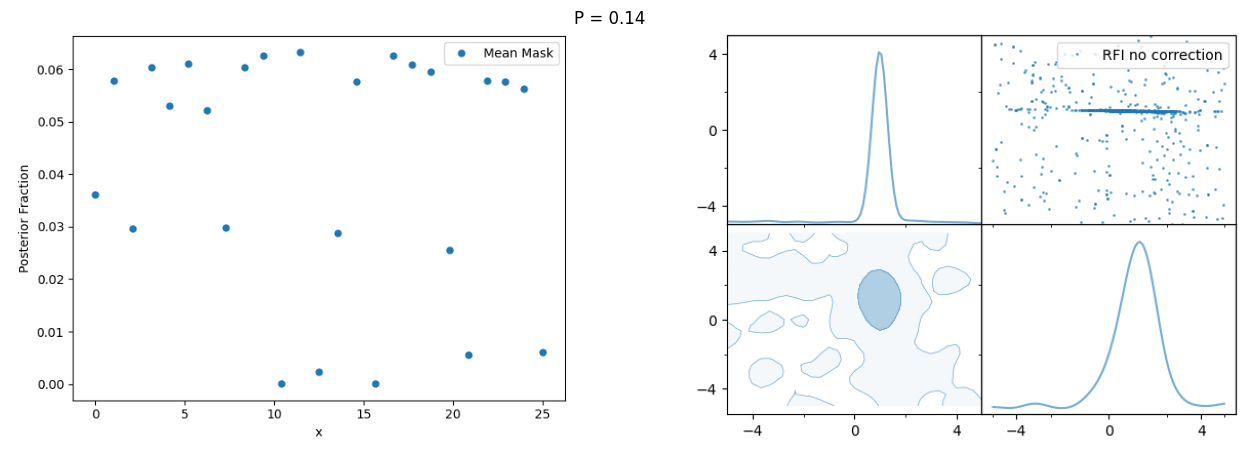
\includegraphics[width=0.8\textwidth]{images/gif_anest/comb_8.png}
\end{frame}

\begin{frame}{Varying $p$}
    \centering
    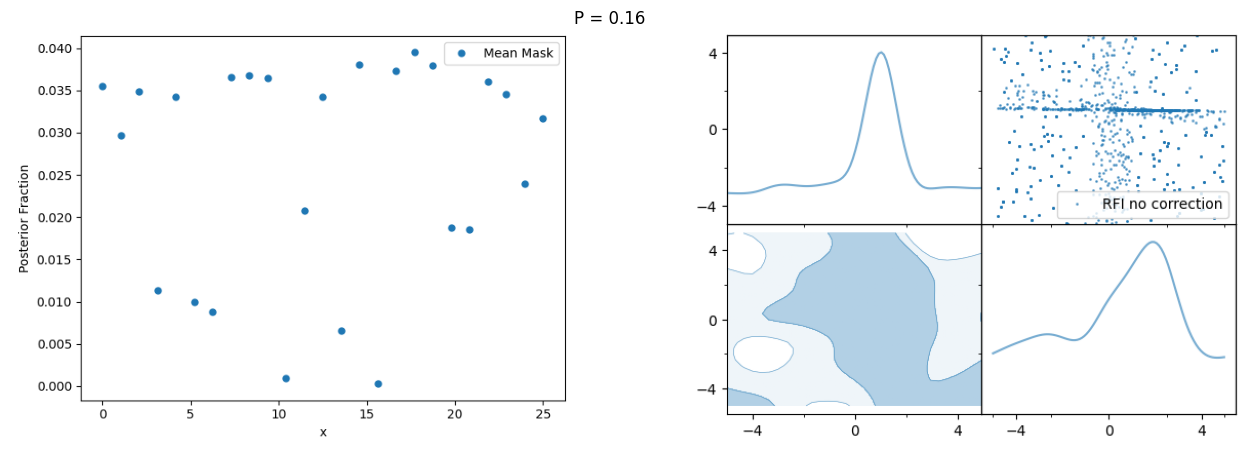
\includegraphics[width=0.8\textwidth]{images/gif_anest/comb_9.png}
\end{frame}


\begin{frame}{Selection strategy for $p$.}
  \begin{columns}
    \column{0.5\textwidth}
    \begin{itemize}
      \item `Select $p$ such that the Bayesian evidence is maximised'
    \end{itemize}
    \column{0.5\textwidth}
    \begin{figure}
      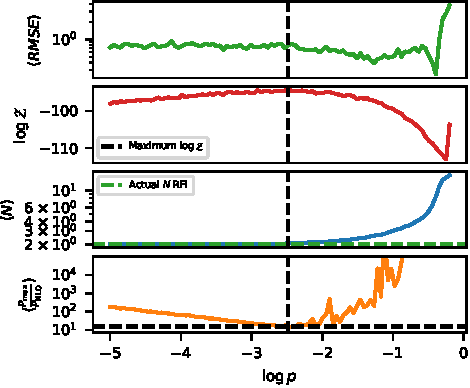
\includegraphics[width=0.8\textwidth]{images/f_approx_current_sig5_2.pdf}
    \end{figure}
  \end{columns}
\end{frame}

\begin{frame}{Fully automated anomaly detection}
  \begin{itemize}
  \item Putting a prior on $p$, we can fit it dynamically as a free parameter.
  \item This fully automates the anomaly detection process.
  \item Must exclude $p=0$.
  \end{itemize}
\end{frame}

\begin{frame}{Application to toy model}
  \centering
  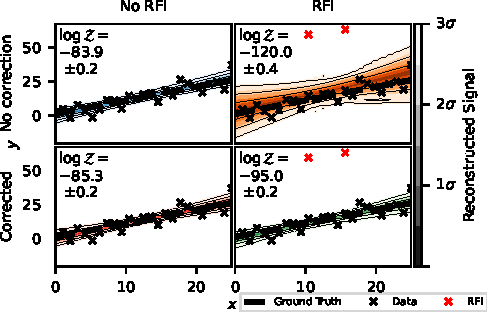
\includegraphics[width=0.64\textwidth]{images/4pane_toy_sidebar.pdf}
\end{frame}

\begin{frame}{Implement with 2 lines of code}
  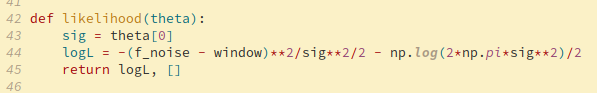
\includegraphics[width=1\textwidth]{images/logl1.png}
  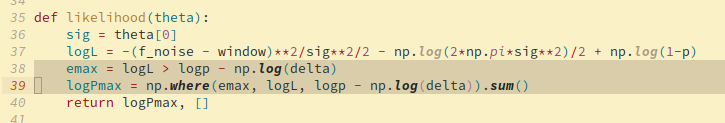
\includegraphics[width=1\textwidth]{images/logl2.png}
  \centering Tutorial @ github.com/samleeney
\end{frame}

\begin{frame}{Read the paper!}
  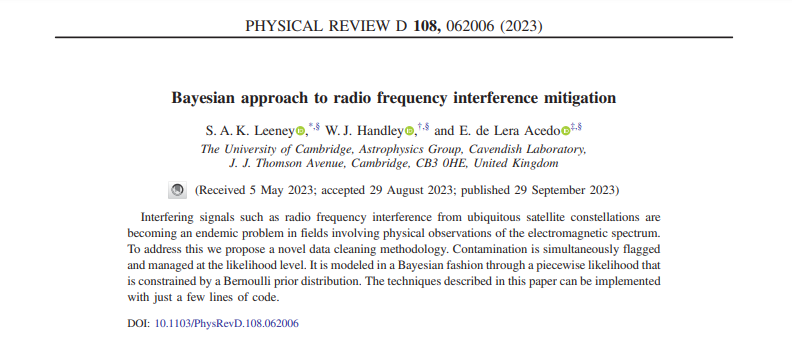
\includegraphics[width=1\textwidth]{images/paper1.png}
  \href{https://arxiv.org/abs/2211.15448}{arxiv: 2211.15448}
\end{frame}

\section{Apply to 21cm Cosmology}

\begin{frame}{What is REACH?}
  \begin{columns}
    \column{0.6\textwidth}
      \centering
      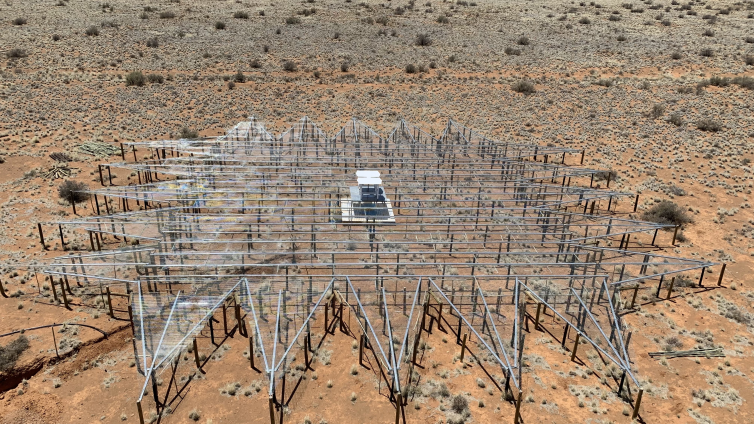
\includegraphics[width=1\textwidth]{images/antenna.png} % Image placeholder
    \column{0.4\textwidth}
      \begin{itemize}
        \item The redshifted sky-averaged 21cm line of neutral hydrogen carries the imprint of the first stars and galaxies formed during the Cosmic Dawn and Epoch of Reionisation
        \item $10^-5$ times dimmer than foregrounds.
        \item Detection enables inference of fundamental physics and cosmology.
      \end{itemize}
  \end{columns}
\end{frame}

\begin{frame}{Heavily contaminated}
  \centering 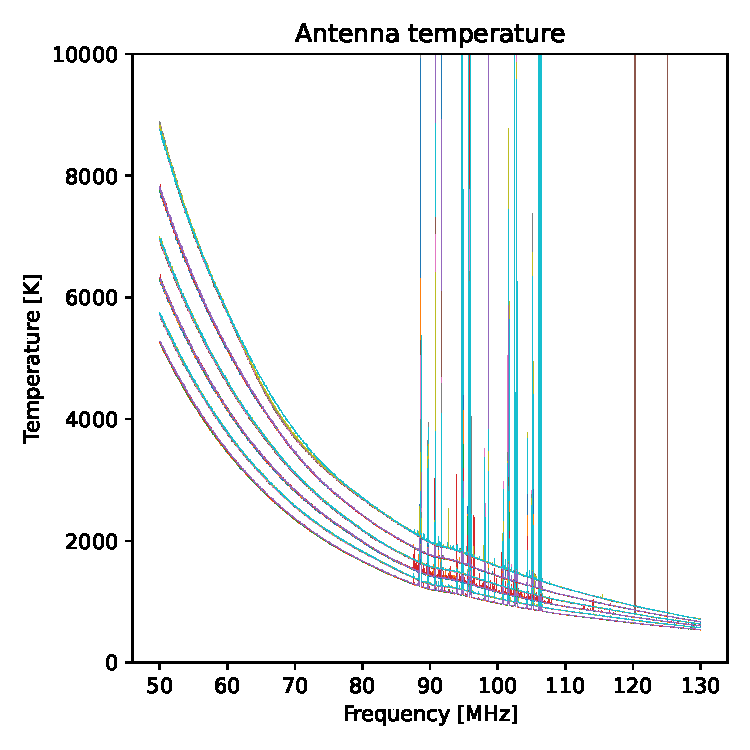
\includegraphics[width=0.5\textwidth]{images/antenna_data_all.pdf}
\end{frame}

\begin{frame}{Fitting a contaminated global 21cm signal}

  \footnotesize
  \begin{columns}
    \column{0.5\textwidth}
    \textbf{Standard Likelihood:}
    \begin{align*}
      \log \mathcal{L} &= \sum_i -\frac{1}{2}\log \left(2\pi\sigma_n^2\right) \\
      &\quad - \frac{1}{2} \left(\frac{T_{\text{data}}(\nu_i) - (T_{\text{model}}(\nu_i) + T_{21}(\nu_i))}{\sigma_n}\right)^2.
    \end{align*}
    \begin{itemize}
      \item $T_{\text{data}}(\nu_i)$: Observed data at frequency $\nu_i$
      \item $T_{\text{model}}(\nu_i)$: Model for foregrounds and nuisance parameters
      \item $T_{21}(\nu_i)$: Global 21cm signal (signal of interest)
      \item $\sigma_n$: Noise uncertainty
    \end{itemize}

    \column{0.5\textwidth}
    \textbf{Anomaly Detection Likelihood:}
    \begin{align*}
      \log \mathcal{L}_{\text{anom}} &= \sum_i \begin{cases}
        \log \mathcal{L}_i + \log(1-p), & \text{if } e_i^{\max} \\
        \log p - \log \Delta, & \text{otherwise}
      \end{cases}
    \end{align*}
    \begin{itemize}
      \item $\log \mathcal{L}_i$: Point-wise standard likelihood
      \item $p$: Anomaly probability (model parameter)
      \item $e_i^{\max}$: Boolean indicating normal data
      \item $\Delta$: Maximum value of the data range
    \end{itemize}
  \end{columns}
\end{frame}

\begin{frame}{Fitting a contaminated global 21cm signal}
  \centering 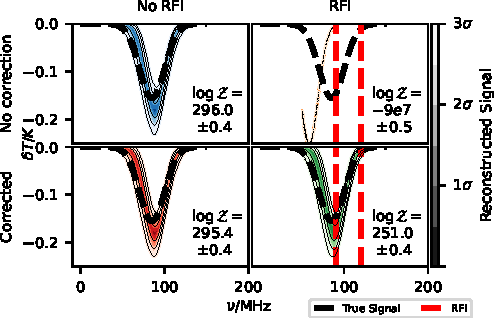
\includegraphics[width=0.8\textwidth]{images/4pane_reach_sidebar.pdf}
\end{frame}

\begin{frame}{Speeding up...}
  \begin{columns}
    \column{0.5\textwidth}
      \centering
      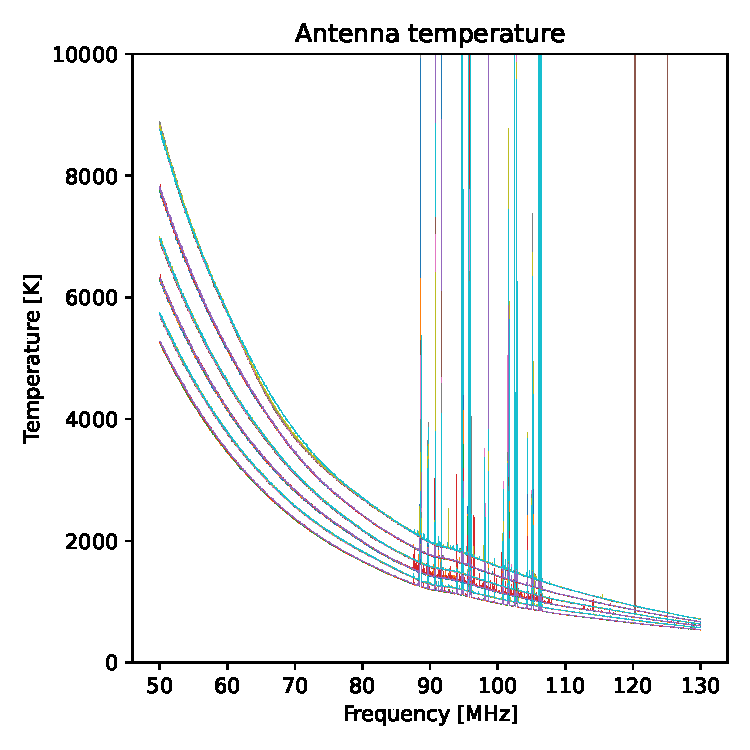
\includegraphics[width=0.9\textwidth]{images/antenna_data_all.pdf} % Adjusted width for column
    \column{0.5\textwidth}
      \begin{itemize}
        \item We fit many observations simultaneously.
        \item This gets very slow, so we need to speed up.
      \end{itemize}
  \end{columns}
\end{frame}

\begin{frame}{Speeding up...}
  \centering 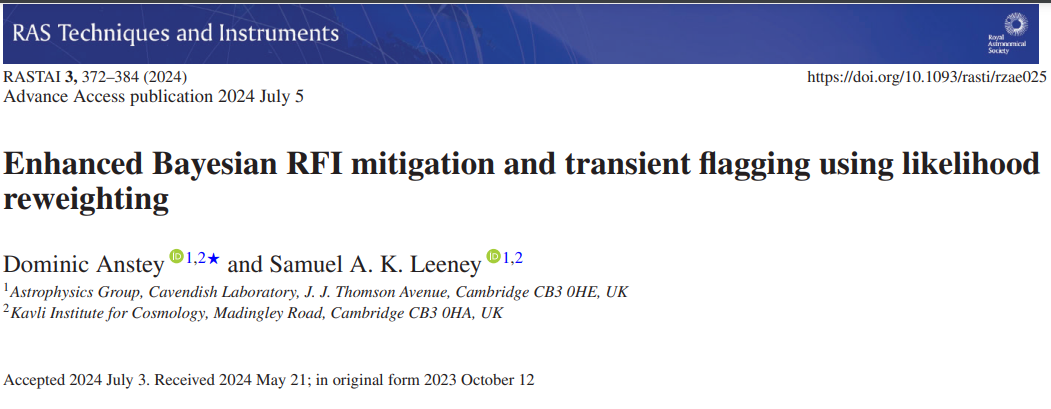
\includegraphics[width=1\textwidth]{images/speedingup.png}
\end{frame}

\section{Apply on Ia supernovae}

\begin{frame}{JAX-bandflux: A Tool for Supernovae Analysis}
  \vfill
  \begin{center}
    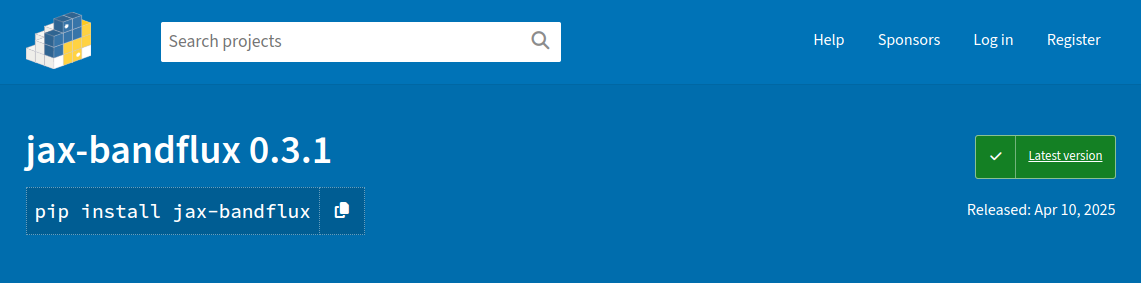
\includegraphics[width=0.64\textwidth]{images/jaxbandflux-pip.png}
  \end{center}
  \vfill
  \begin{center}
    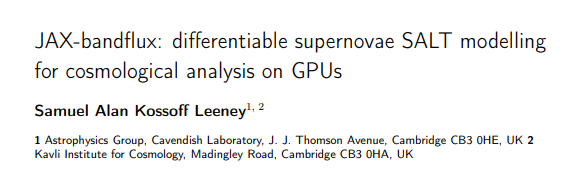
\includegraphics[width=0.64\textwidth]{images/jaxbandflux-paper.png}
  \end{center}
  \vfill
\end{frame}
\begin{frame}{JAX-bandflux: A Tool for Supernovae Analysis}
  \centering 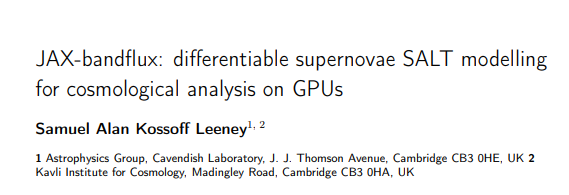
\includegraphics[width=0.8\textwidth]{images/josjaxbflux.png}
\end{frame}
\begin{frame}{Fitting Supernovae Light Curves with \texttt{JAX-bandflux}}
  \begin{columns}
    \column{0.5\textwidth}
      \begin{itemize}
        \item Supernovae light curves measure the brightness of a supernova over time across different wavelengths.
        \item \texttt{JAX-bandflux} is a Python package for fitting supernova light curves.
        \item It provides tools for model definition, fitting, and simulation.
        \item GPU acceleration significantly speeds up the fitting process for large datasets.
      \end{itemize}
    \column{0.5\textwidth}
      \centering
      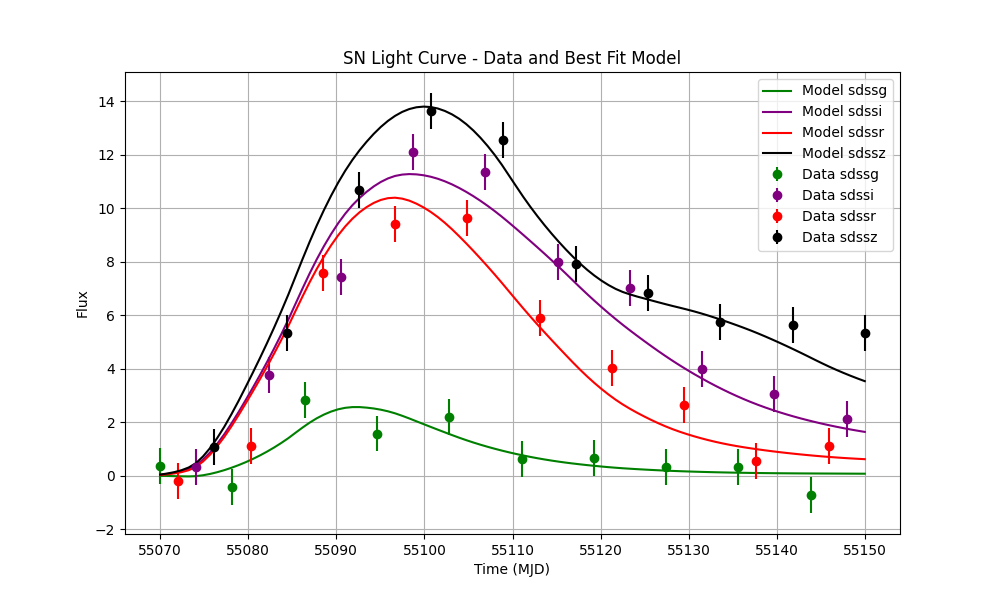
\includegraphics[width=0.9\textwidth]{images/sncosmo-fitter.png}
  \end{columns}
\end{frame}

\begin{frame}{The SALT Model for Supernovae}
  \begin{columns}
    \column{0.5\textwidth}
      \begin{itemize}
        \item Widely used empirical model for Type Ia supernovae light curves.
        \item Describes supernova flux as a function of wavelength and time.
      \end{itemize}
    \column{0.5\textwidth}
      \centering
      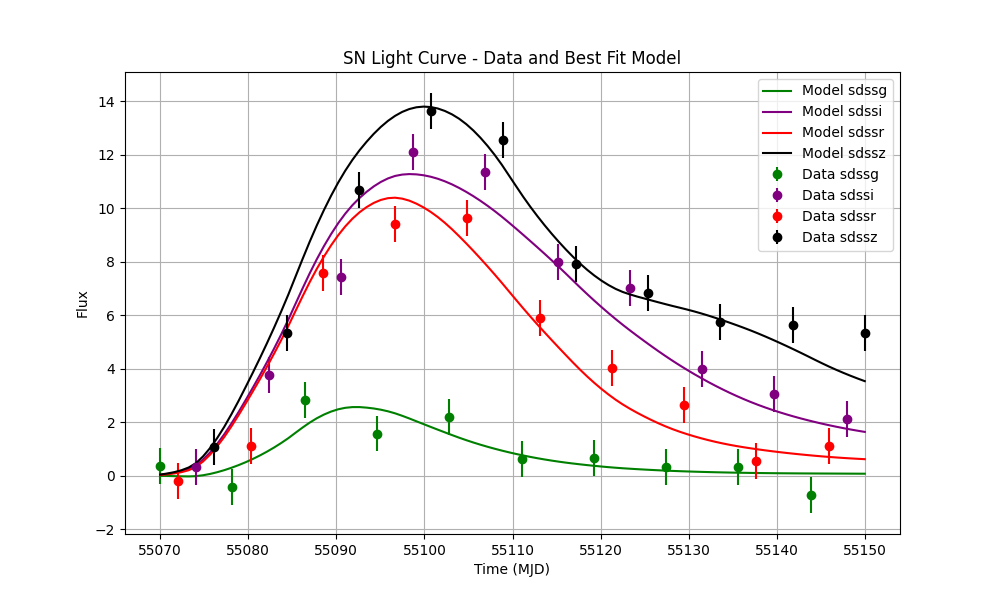
\includegraphics[width=0.9\textwidth]{images/sncosmo-fitter.png}
  \end{columns}
  \vfill % Add vertical fill to push content downwards
  \centering % Center the subsequent content
  Model flux:
  \begin{equation*}
    F(p, \lambda) = x_0 \left[M_0(p, \lambda) + x_1M_1(p, \lambda) + \dots\right] \times \exp \left[c \times CL(\lambda)\right]
  \end{equation*}
\end{frame}

\begin{frame}{Bandflux Computation}
  \begin{columns}
    \column{0.5\textwidth}
      \begin{itemize}
        \item Observed flux integrated over a specific photometric bandpass.
        \item Calculated by convolving SED with instrument's bandpass transmission.
        \item Formula:
          \begin{equation*}
            \text{bandflux} = \int_{\lambda_{\text{min}}}^{\lambda_{\text{max}}} F(\lambda) \cdot T(\lambda) \cdot \frac{\lambda}{hc} d\lambda
          \end{equation*}
      \end{itemize}
    \column{0.5\textwidth}
      \centering
      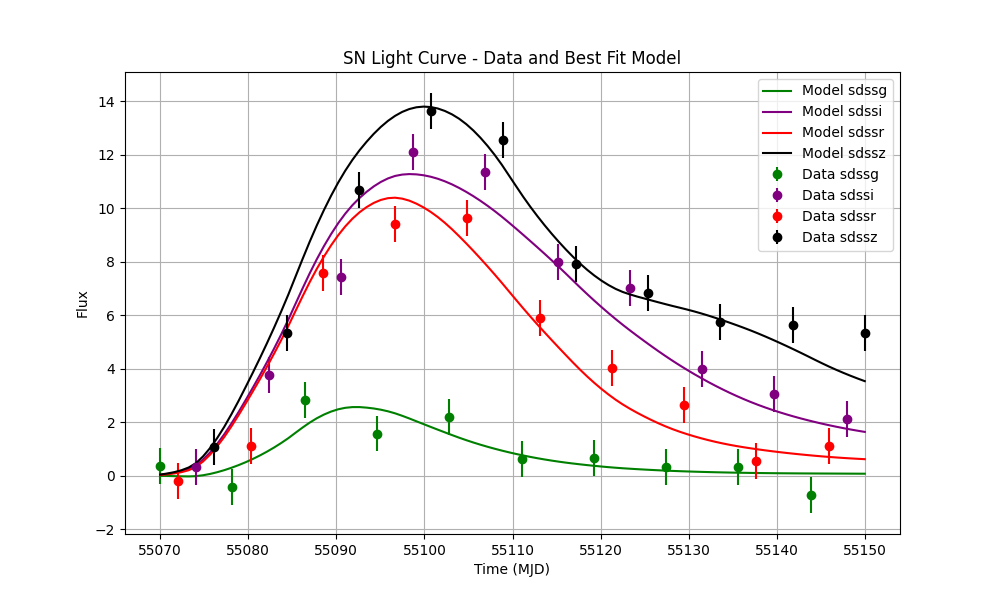
\includegraphics[width=0.9\textwidth]{images/sncosmo-fitter.png}
  \end{columns}
\end{frame}

\begin{frame}{Cosmology from SALT parameters}
  \begin{itemize}
    \item SALT parameters ($x_0, x_1, c$) are fitted to Type Ia supernovae light curves.
    \item These parameters standardize SNe Ia into standard candles by correcting for luminosity, shape ($x_1$), and color ($c$).
    \item This standardization allows for precise calculation of distance moduli, linking to luminosity distance.
    \item By fitting cosmological models to a large sample of these calibrated supernova distances, cosmological parameters, such as the Hubble constant ($H_0$), can be determined.
  \end{itemize}
\end{frame}


\begin{frame}{Likelihood Function for Supernovae Fitting}
  \begin{itemize}
    \item The likelihood function quantifies how well a given model (e.g., SALT) explains the observed data.
    \item For photometric observations, assuming Gaussian uncertainties, the likelihood is typically defined as:
      \begin{equation*}
        \mathcal{L}(\theta) = \prod_{i=1}^{N} \frac{1}{\sqrt{2\pi\sigma_i^2}} \exp\left(-\frac{(f_i^{\text{obs}} - f_i^{\text{model}}(\theta))^2}{2\sigma_i^2}\right)
      \end{equation*}
      where $f_i^{\text{obs}}$ are observed fluxes, $f_i^{\text{model}}(\theta)$ are model fluxes, and $\sigma_i$ are uncertainties.
    \item In a Bayesian context, this likelihood is combined with priors on the model parameters to form the posterior distribution.
    \item GPU compatibility allows for rapid evaluation of the likelihood across a large parameter space, enabling efficient sampling and inference.
  \end{itemize}
\end{frame}


\begin{frame}{Standard vs. Anomaly Detection Likelihoods}
  \begin{columns}
    \column{0.5\textwidth}
    \textbf{Standard Likelihood:}
    \begin{align}
      \log \mathcal{L}_{\text{std}} &= -\frac{1}{2}\sum_i \left(\frac{f_i - m_i}{\sigma_i}\right)^2 \nonumber \\
      &- \frac{1}{2}\sum_i \log(2\pi\sigma_i^2)
    \end{align}
    \begin{itemize}
      \item $f_i$: Observed flux
      \item $m_i$: Model flux (SALT3)
      \item $\sigma_i$: Flux uncertainty
    \end{itemize}
    
    \column{0.5\textwidth}
    \textbf{Anomaly Detection Likelihood:}
    \begin{align}
      \log \mathcal{L}_{\text{anom}} &= \sum_i \begin{cases}
        \log \mathcal{L}_i + \log(1-p), & \text{if } e_i^{\max} \\
        \log p - \log \Delta, & \text{otherwise}
      \end{cases}
    \end{align}
    \begin{itemize}
      \item $\log \mathcal{L}_i$: Point-wise standard likelihood
      \item $p$: Anomaly probability (fitted parameter)
      \item $e_i^{\max}$: Boolean indicating normal data
      \item $\Delta$: Maximum flux range
    \end{itemize}
  \end{columns}
  
\end{frame}
\begin{frame}{Applying to Ia supernovae}
\begin{center}
  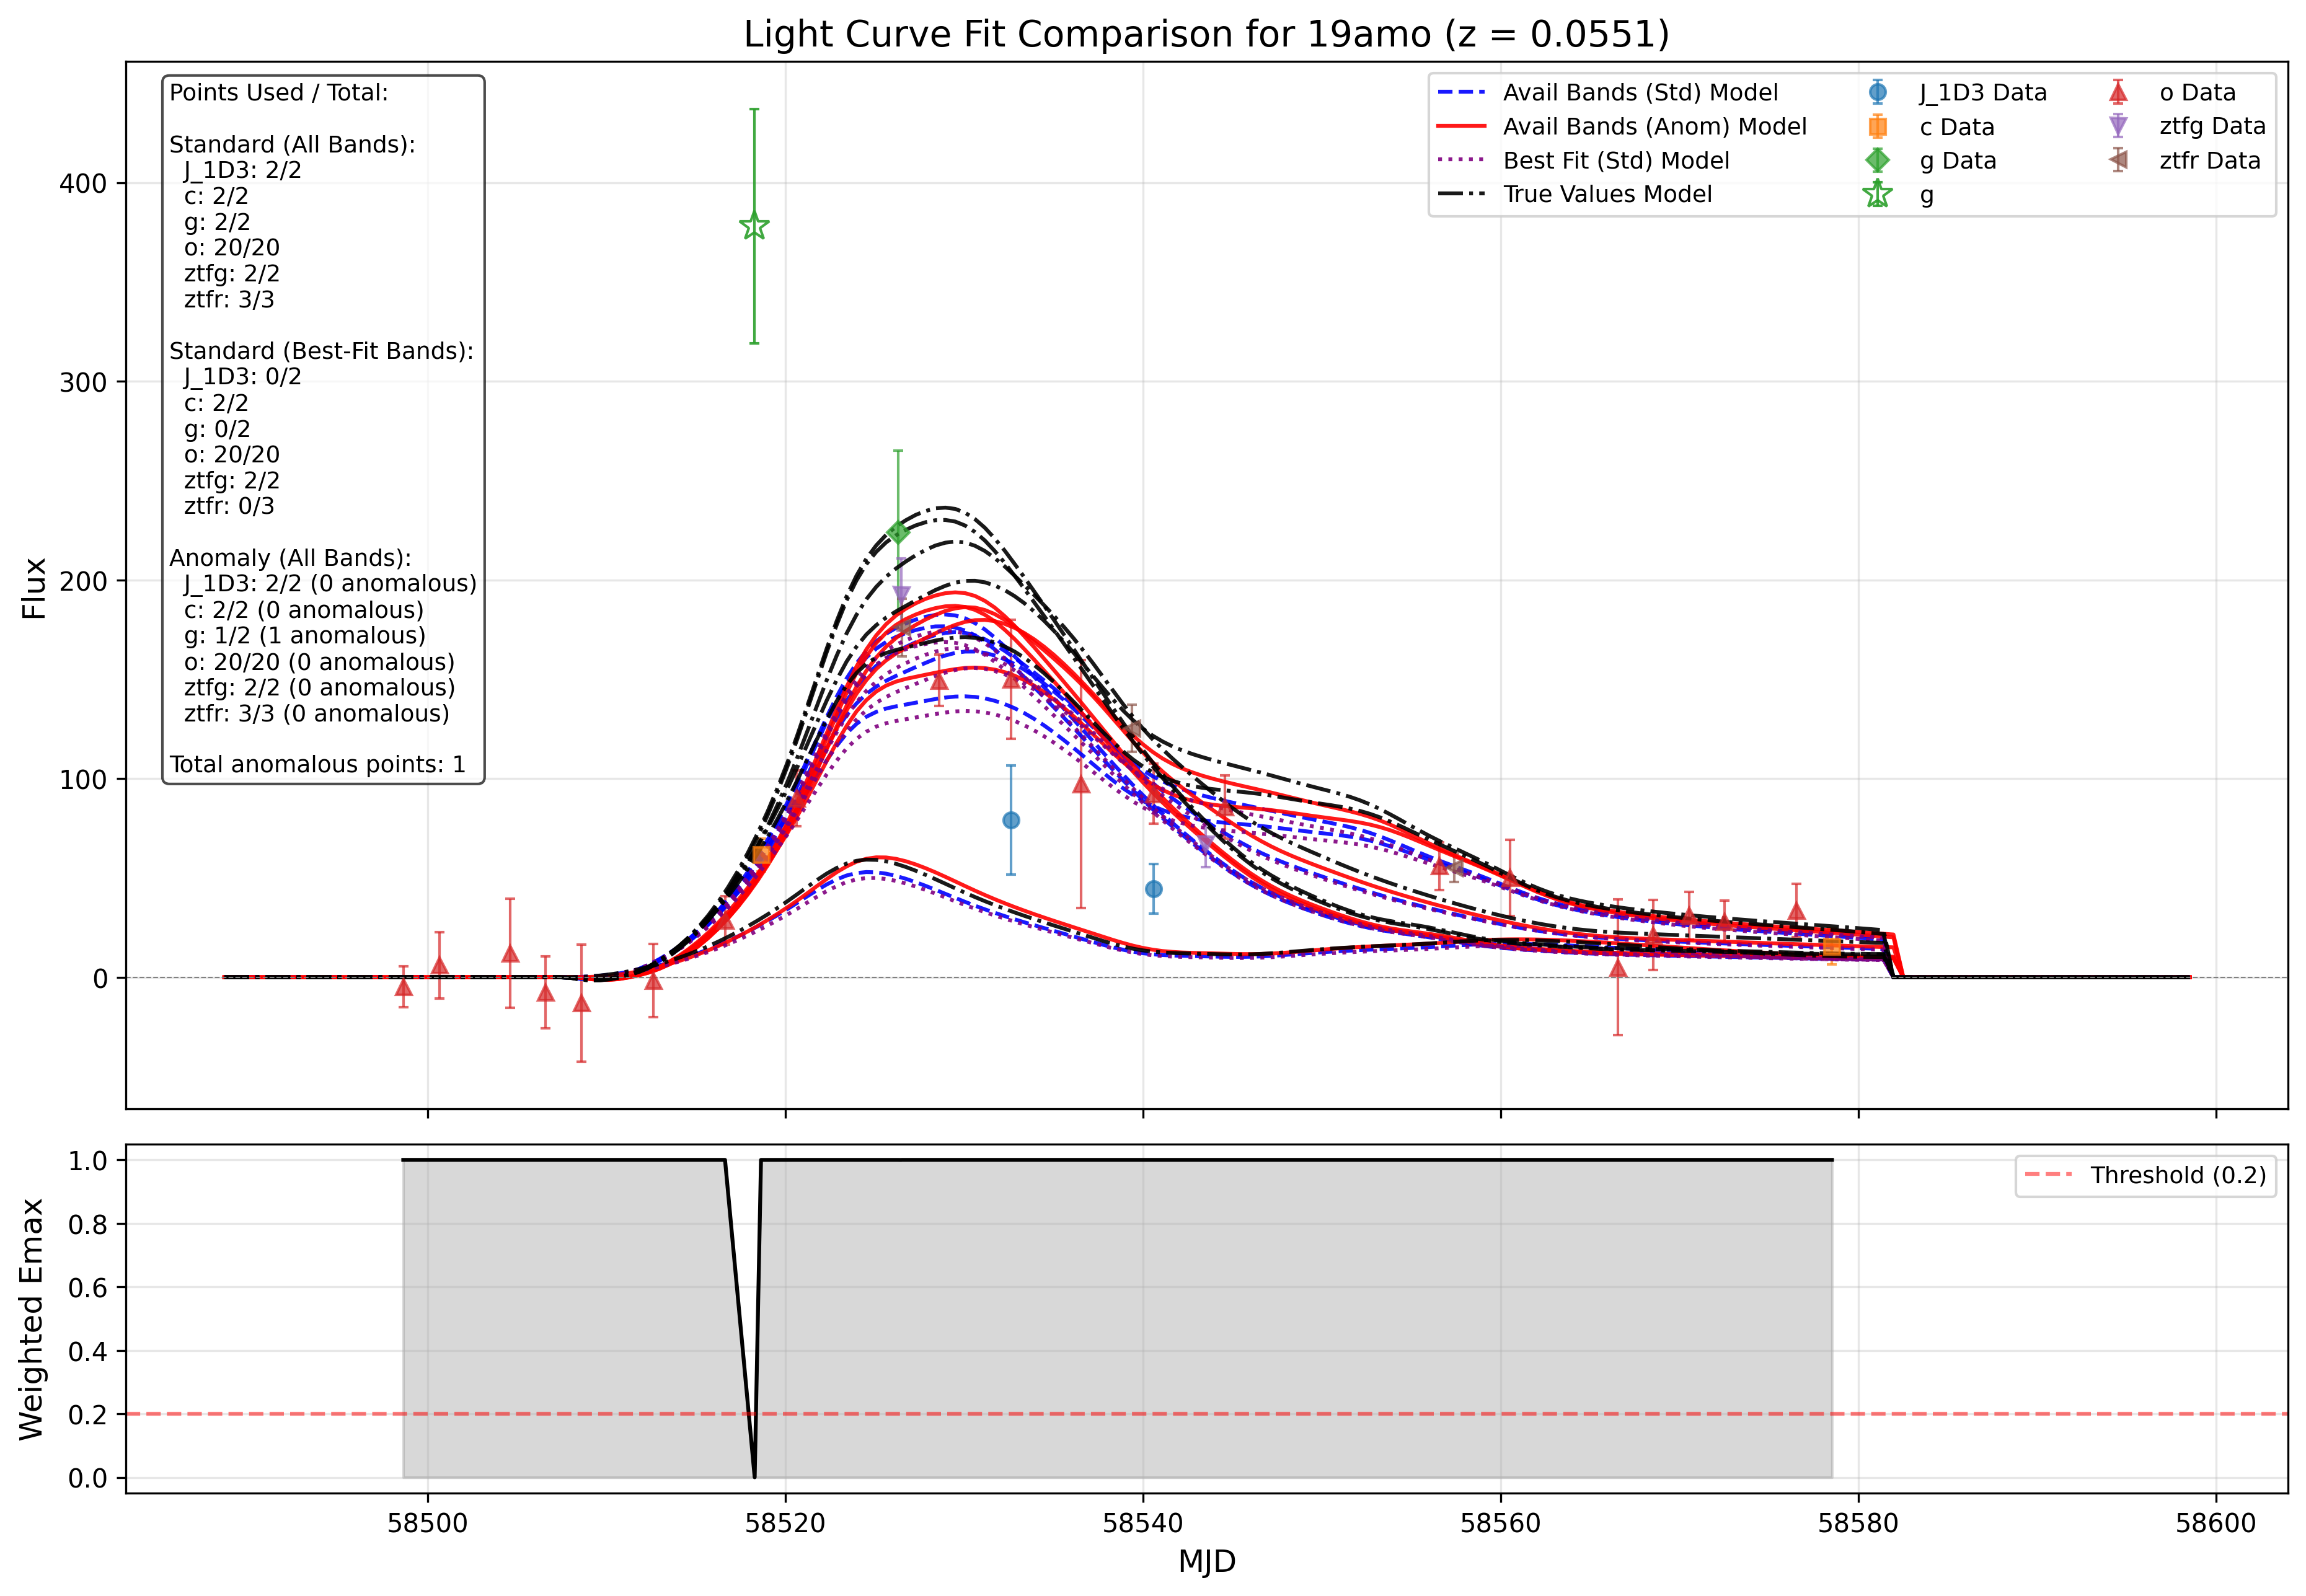
\includegraphics[width=0.64\textwidth]{images/light_curve_comparison_19amo.png}
\end{center}
\end{frame}



\begin{frame}{SN 19amo: Classic 'anomaly detection' example}
  \begin{columns}
    \column{0.5\textwidth}
    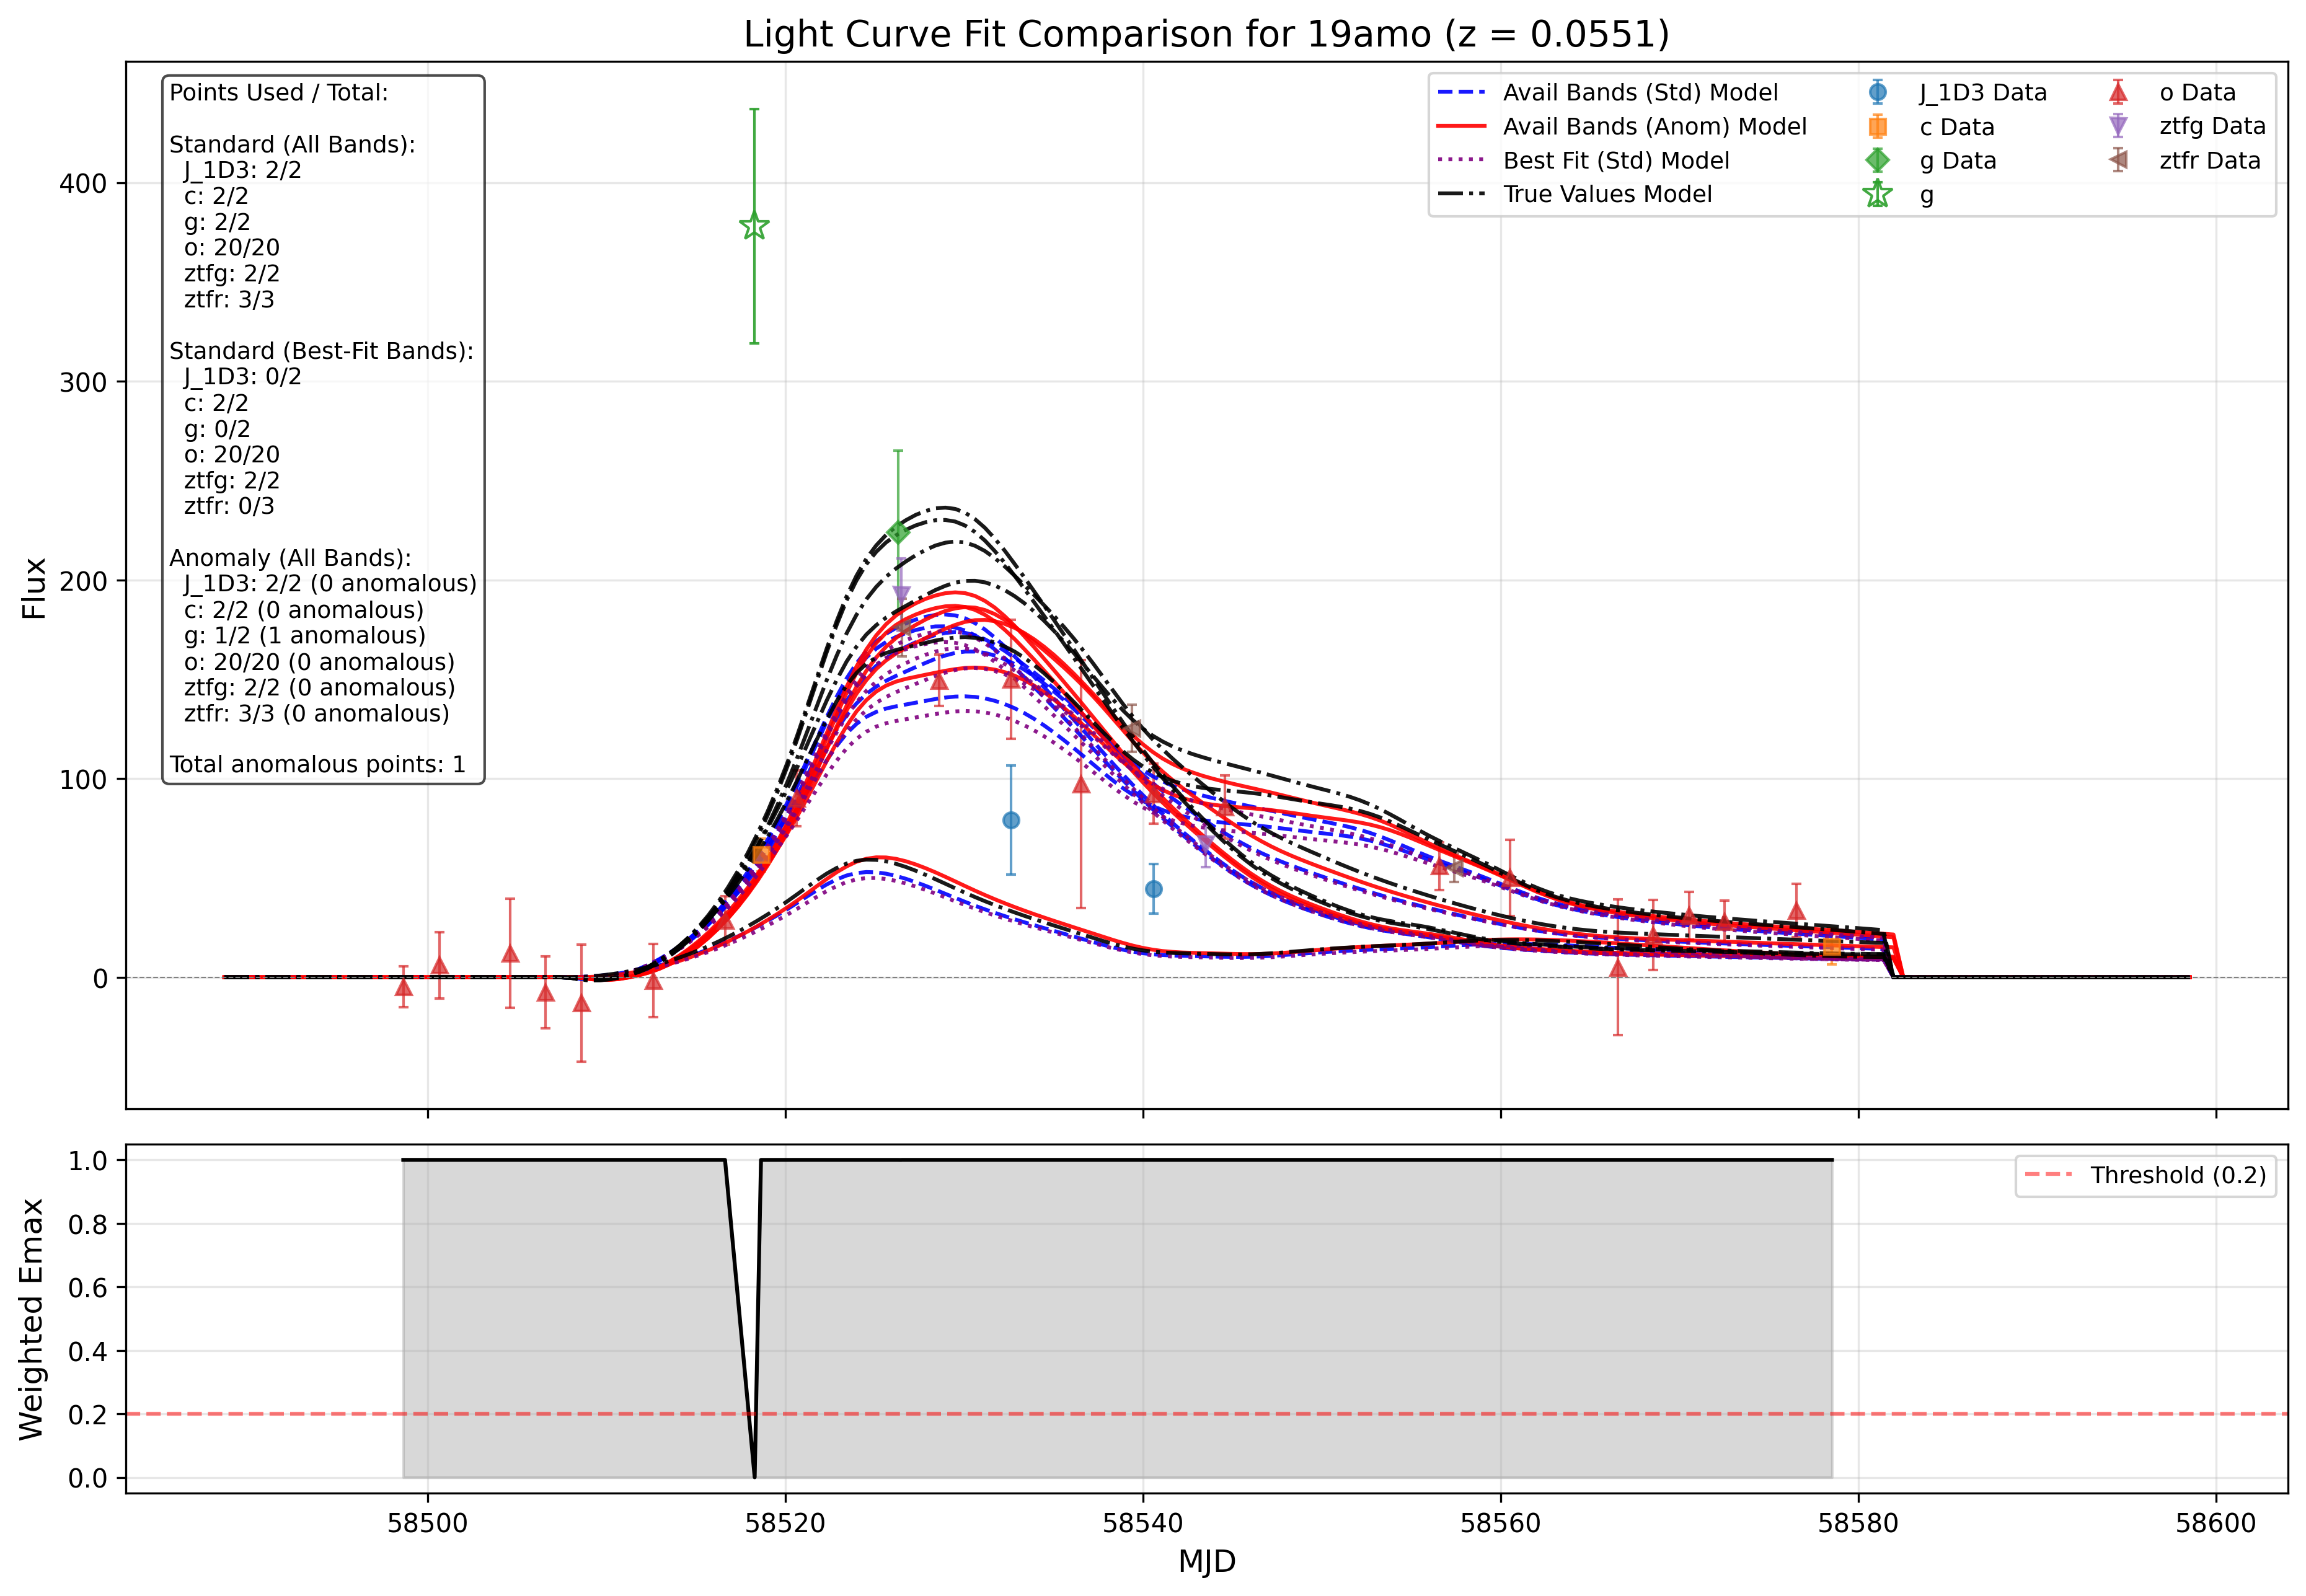
\includegraphics[width=1\textwidth]{images/light_curve_comparison_19amo.png}
    \column{0.5\textwidth}
    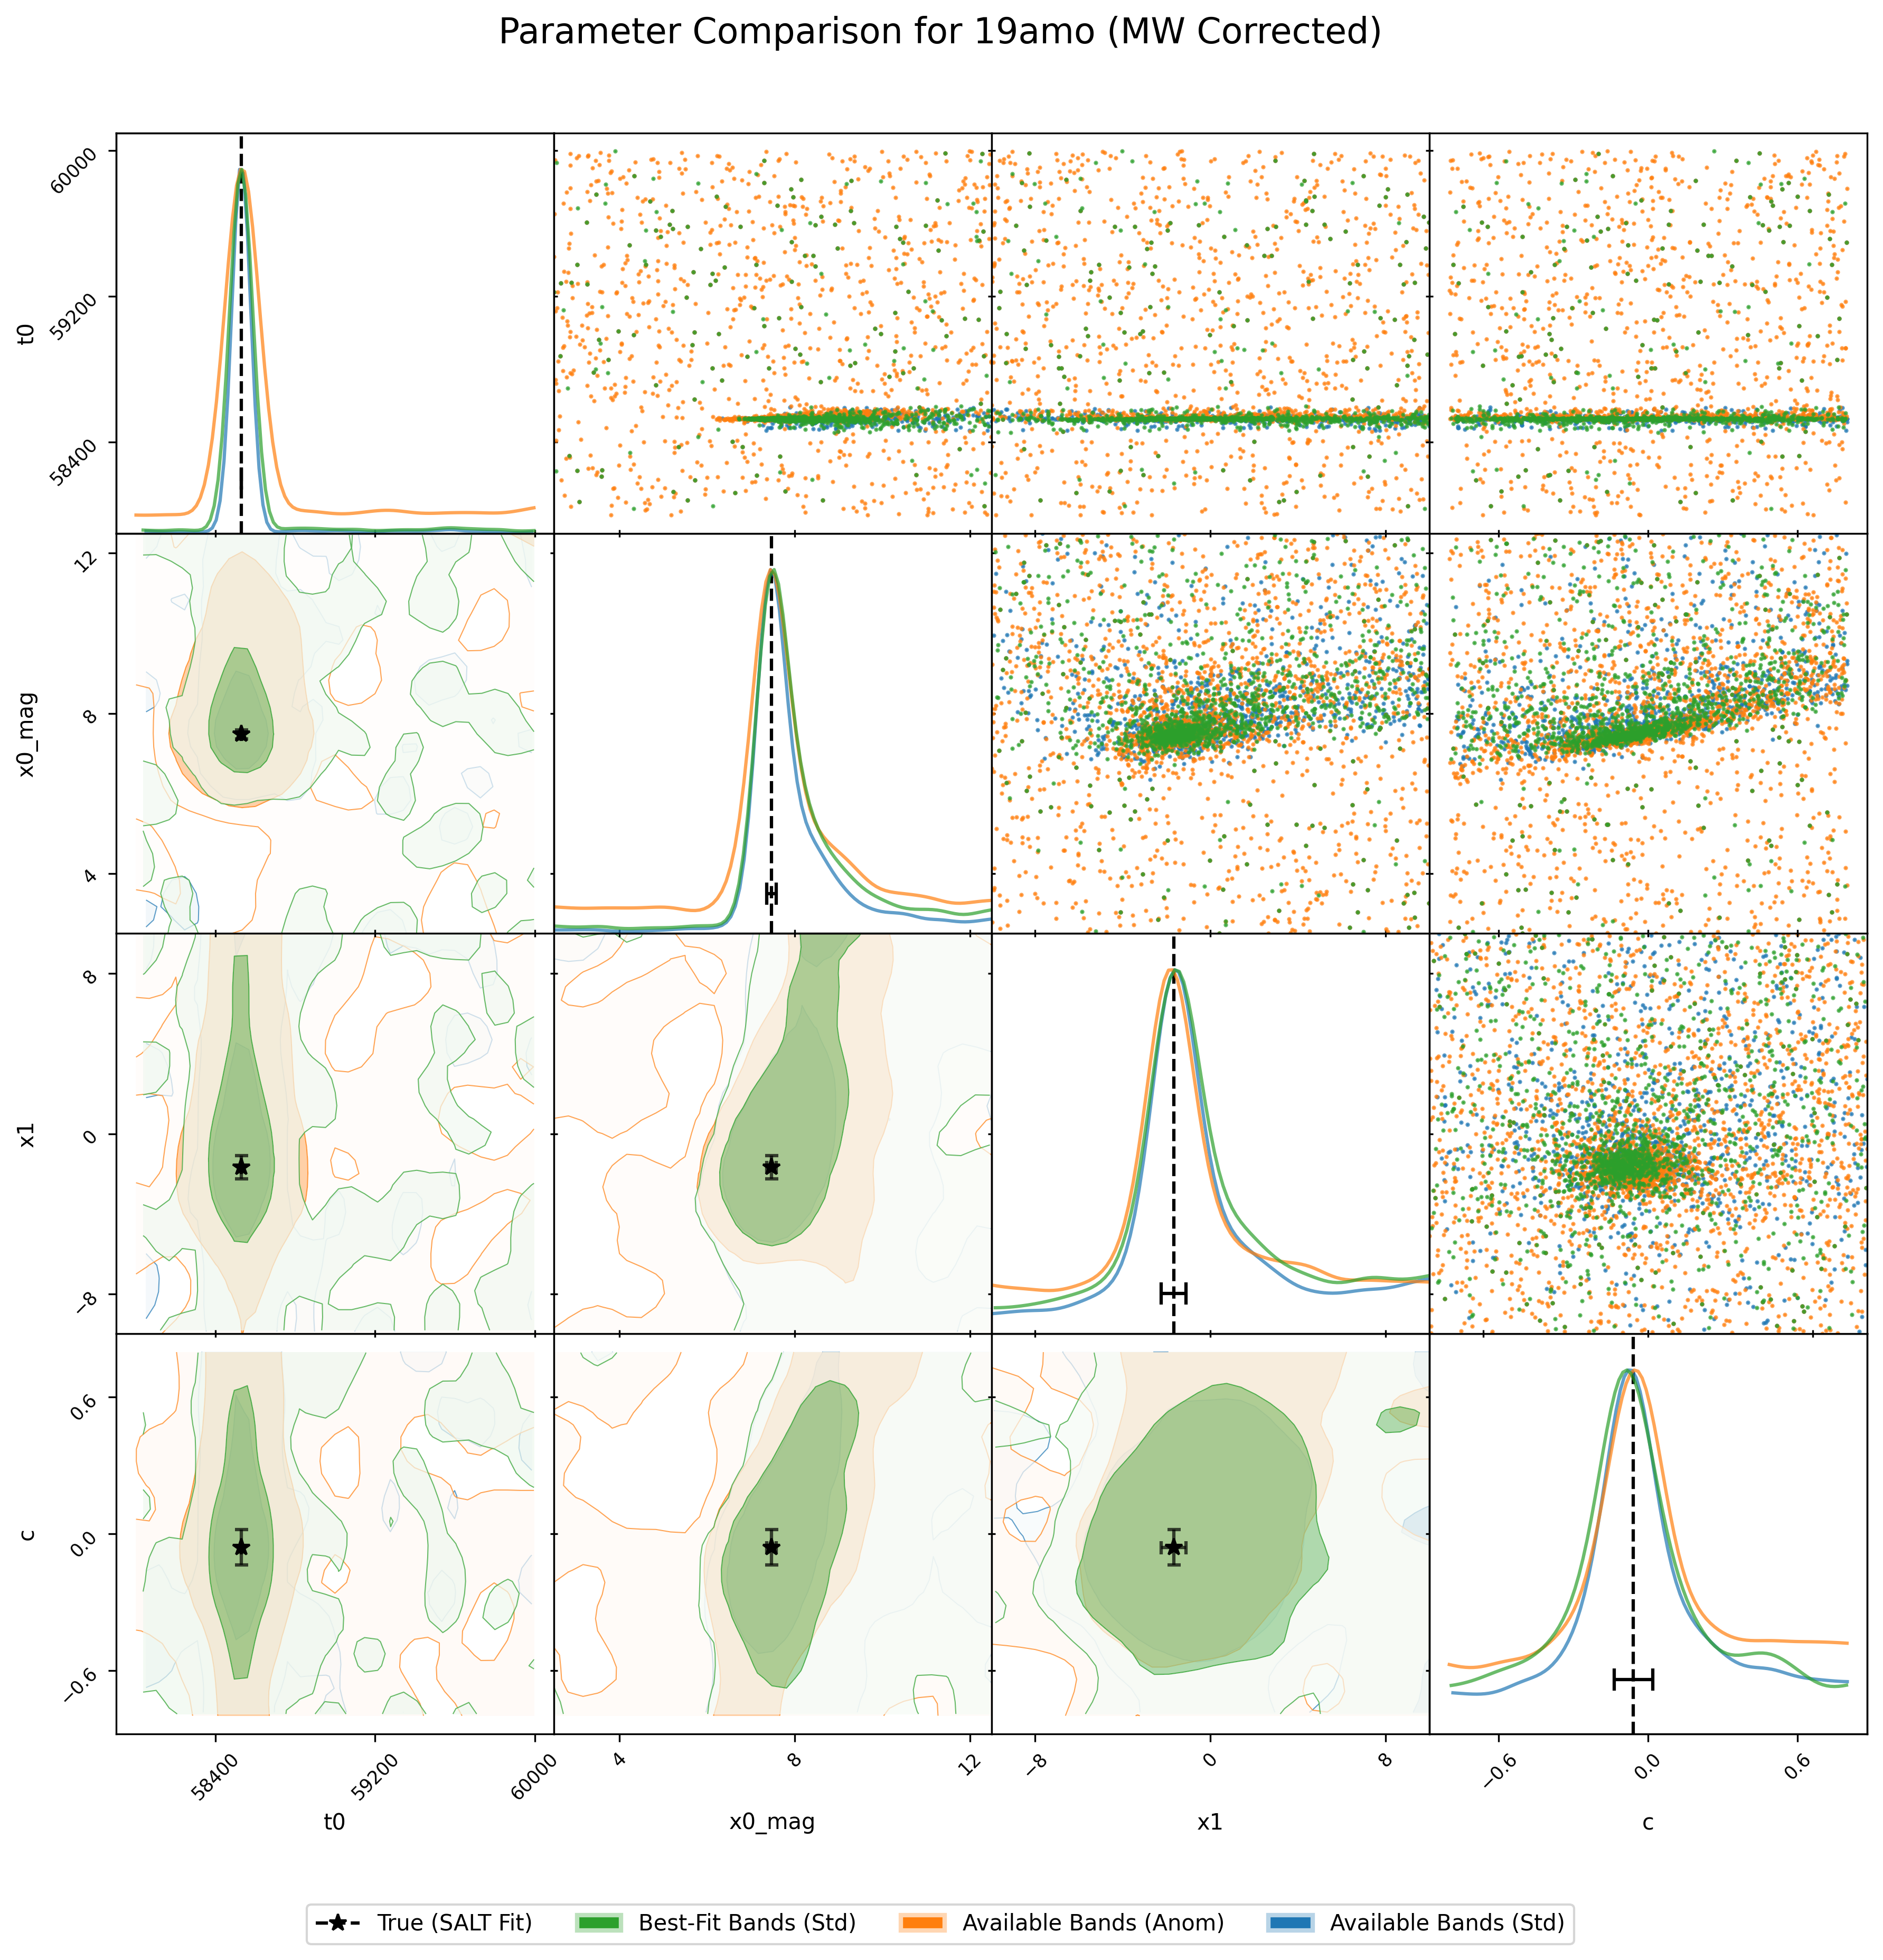
\includegraphics[width=1\textwidth]{images/corner_comparison_19amo.png}
  \end{columns}
\end{frame}

\begin{frame}{SN 19vnk: Automatic filter removal}
  \begin{columns}
    \column{0.5\textwidth}
    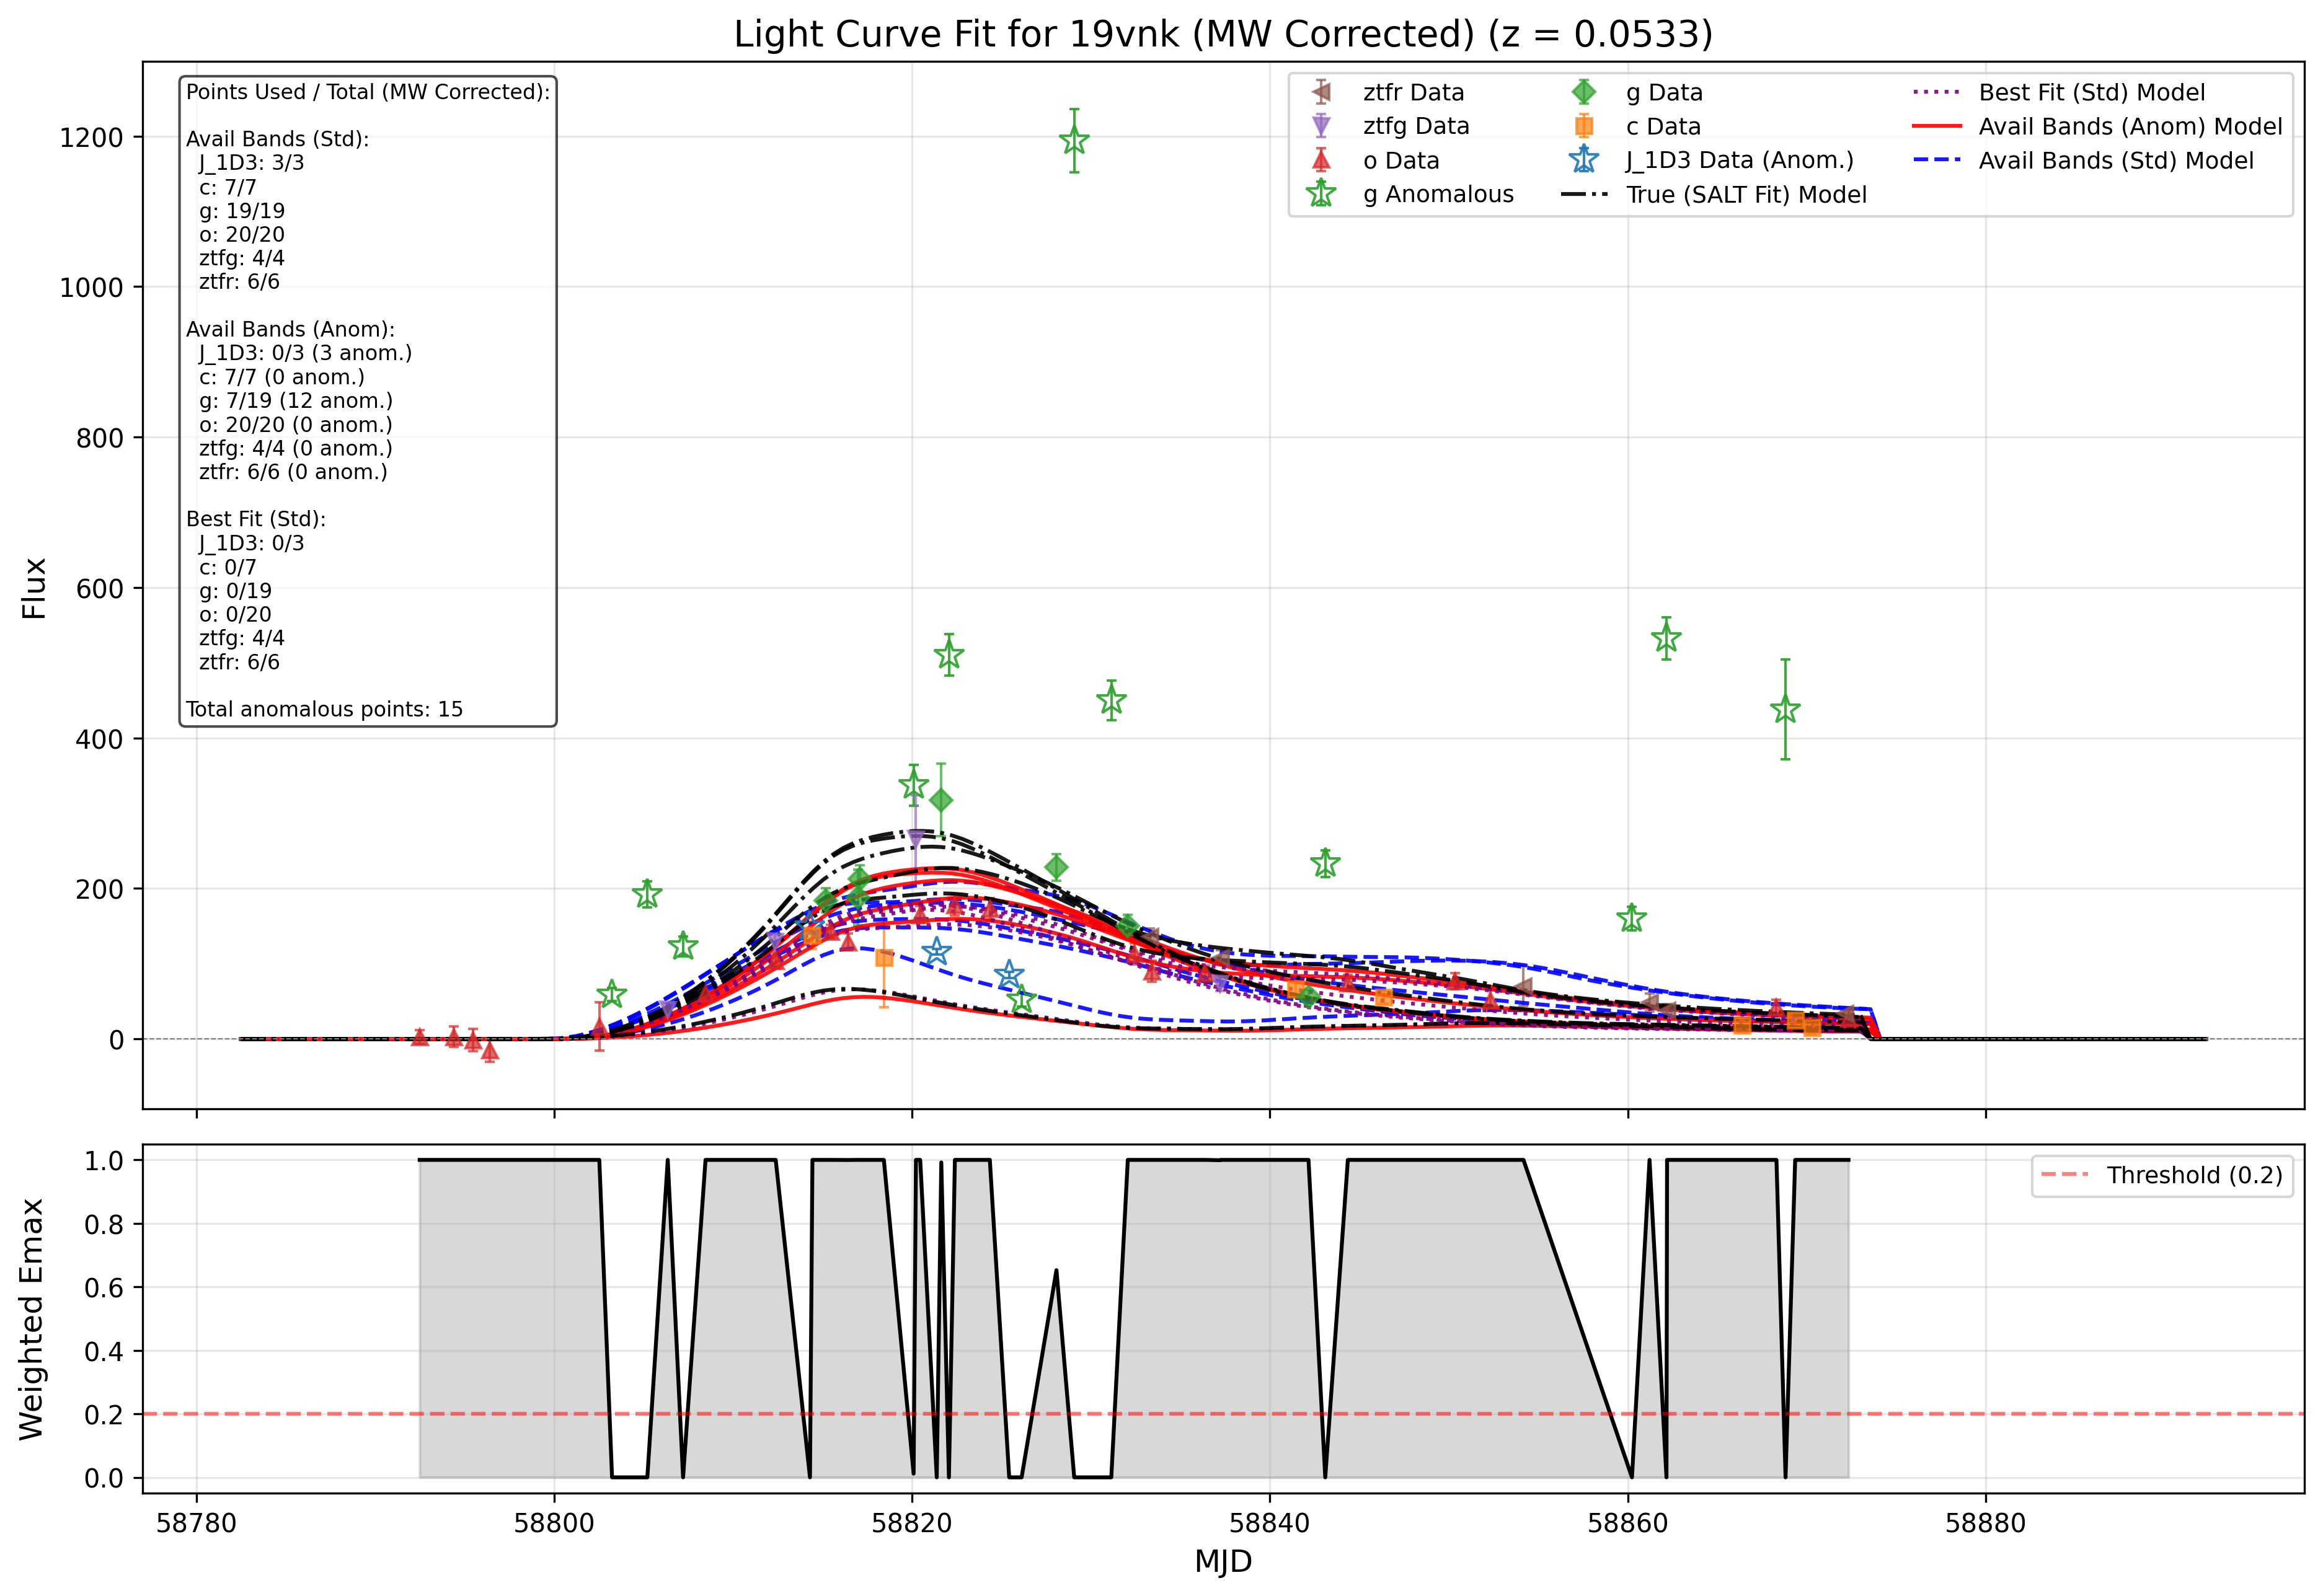
\includegraphics[width=1\textwidth]{images/light_curve_comparison_19vnk.png}
    \column{0.5\textwidth}
    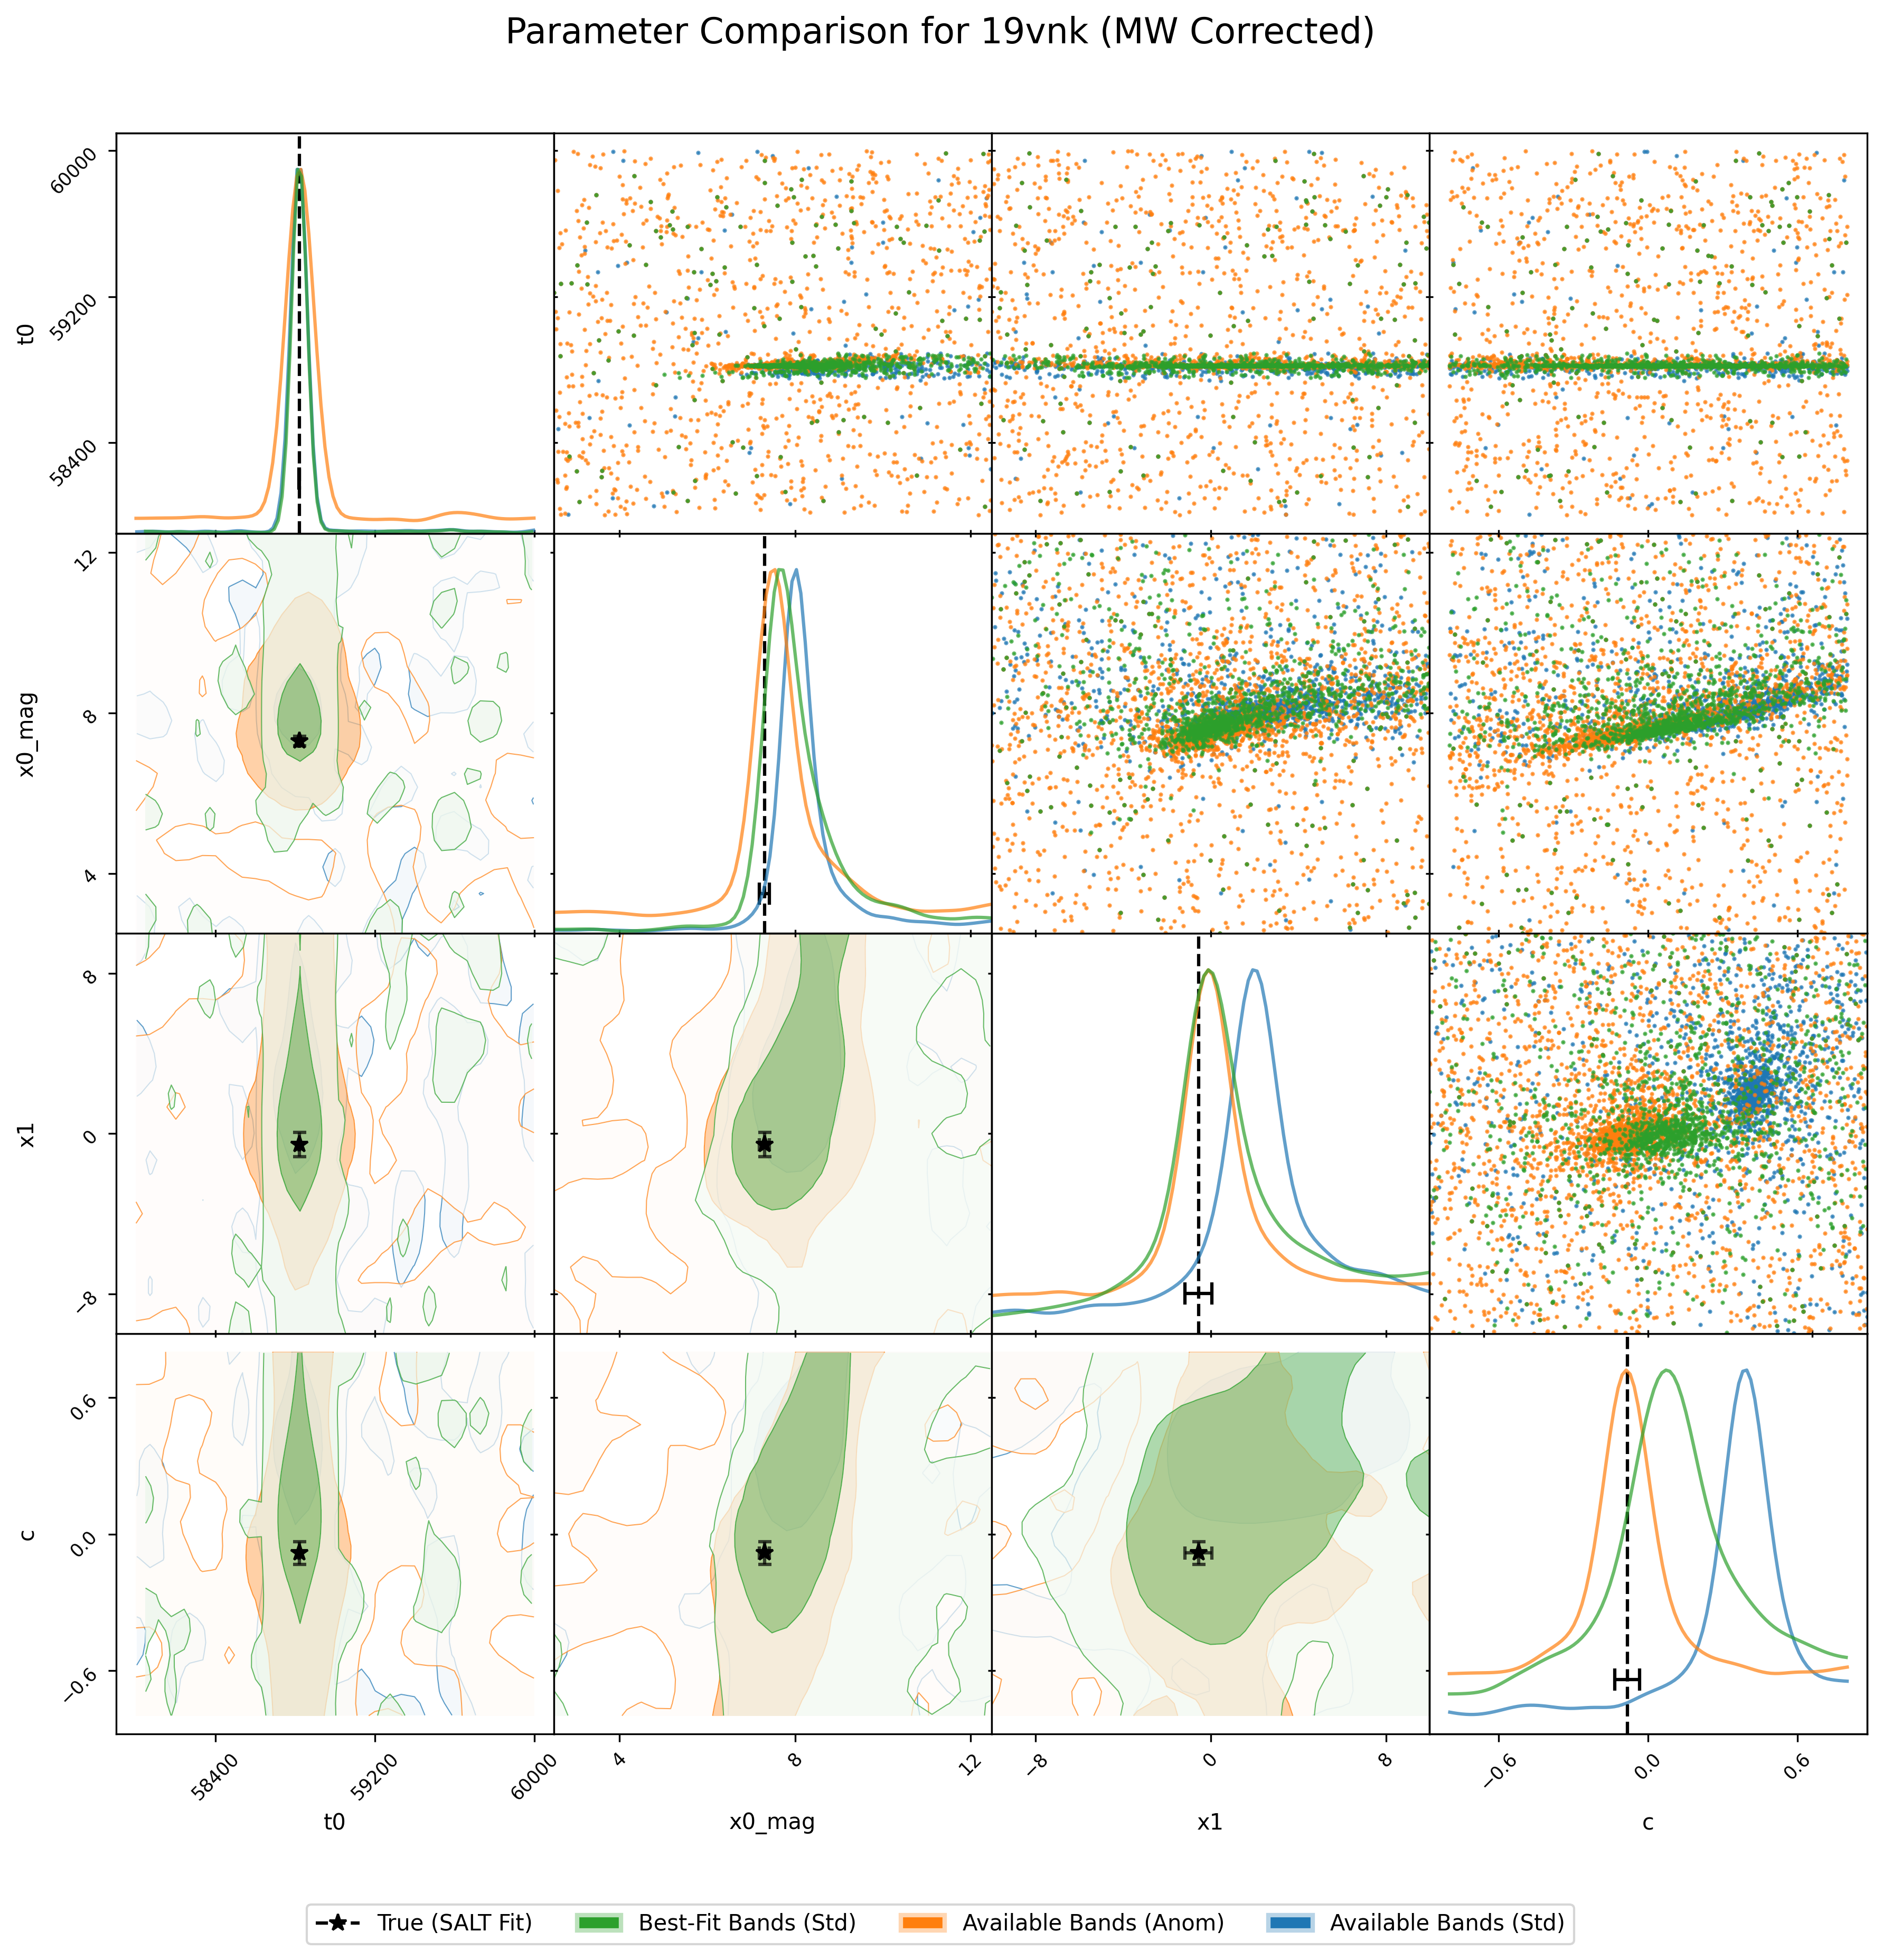
\includegraphics[width=1\textwidth]{images/corner_comparison_19vnk.png}
  \end{columns}
\end{frame}

\begin{frame}{SN 19kai: Flagging while preserving some data}
  \begin{columns}
    \column{0.5\textwidth}
    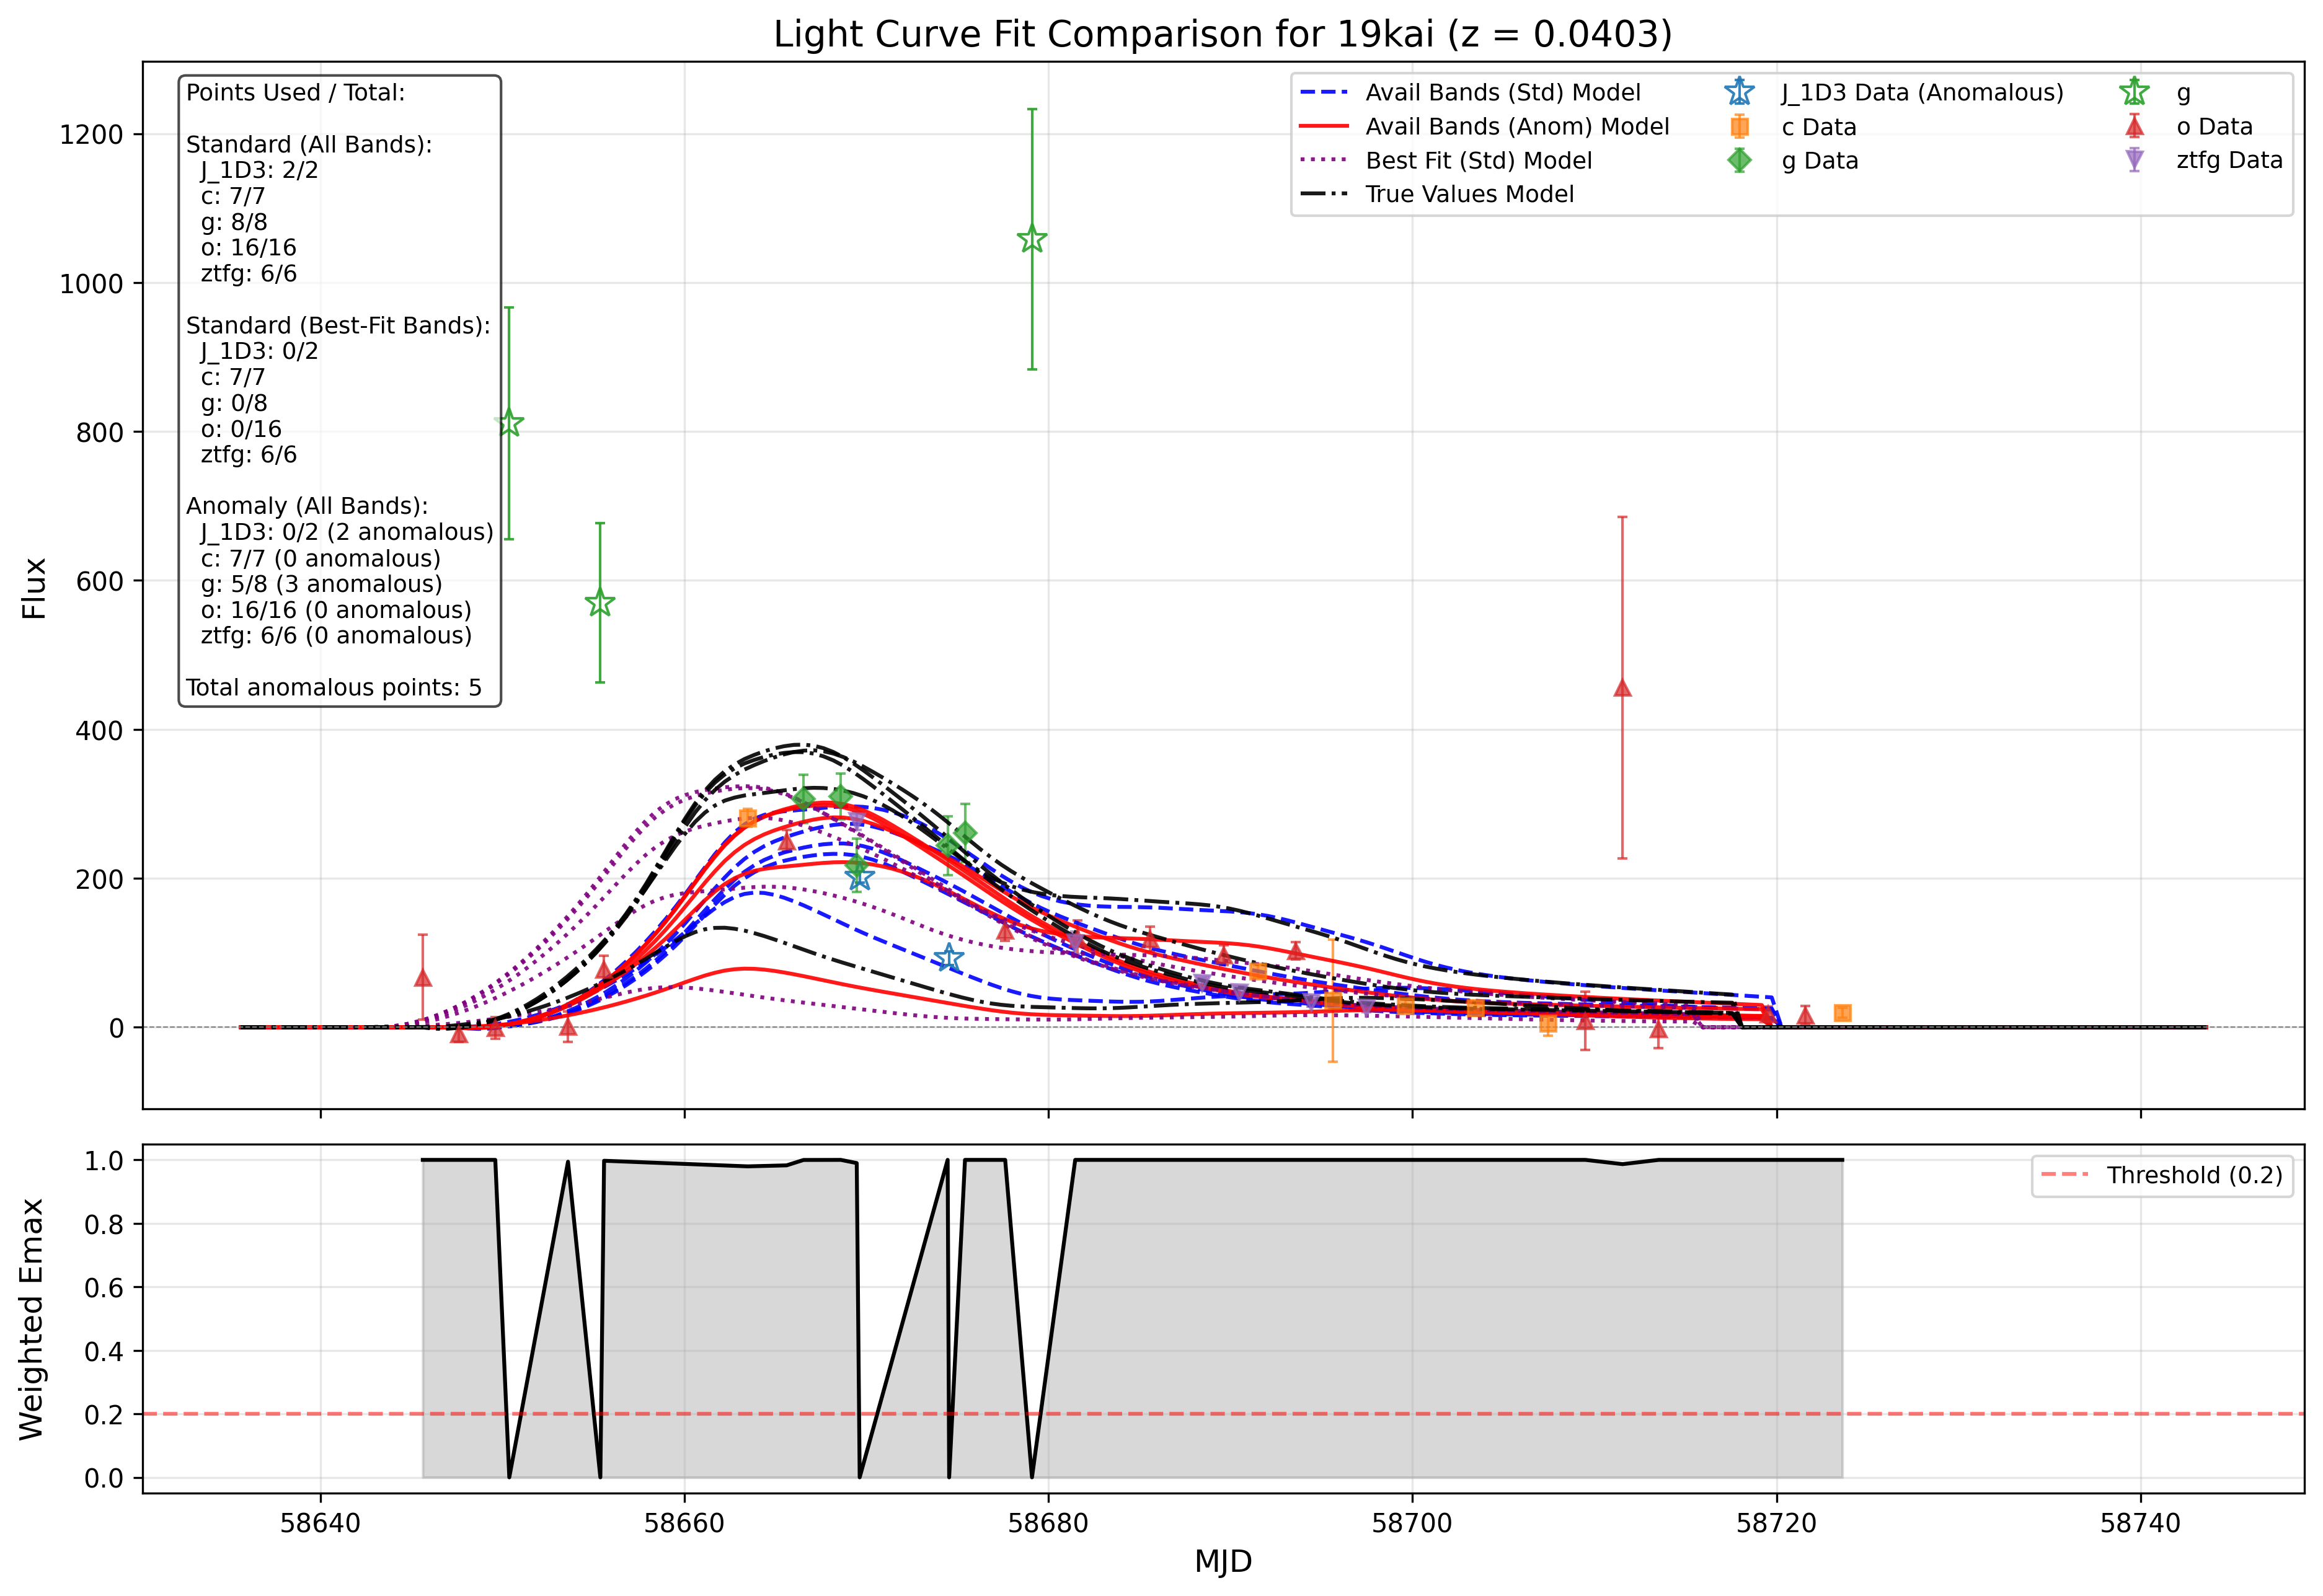
\includegraphics[width=1\textwidth]{images/light_curve_comparison_19kai.png}
    \column{0.5\textwidth}
    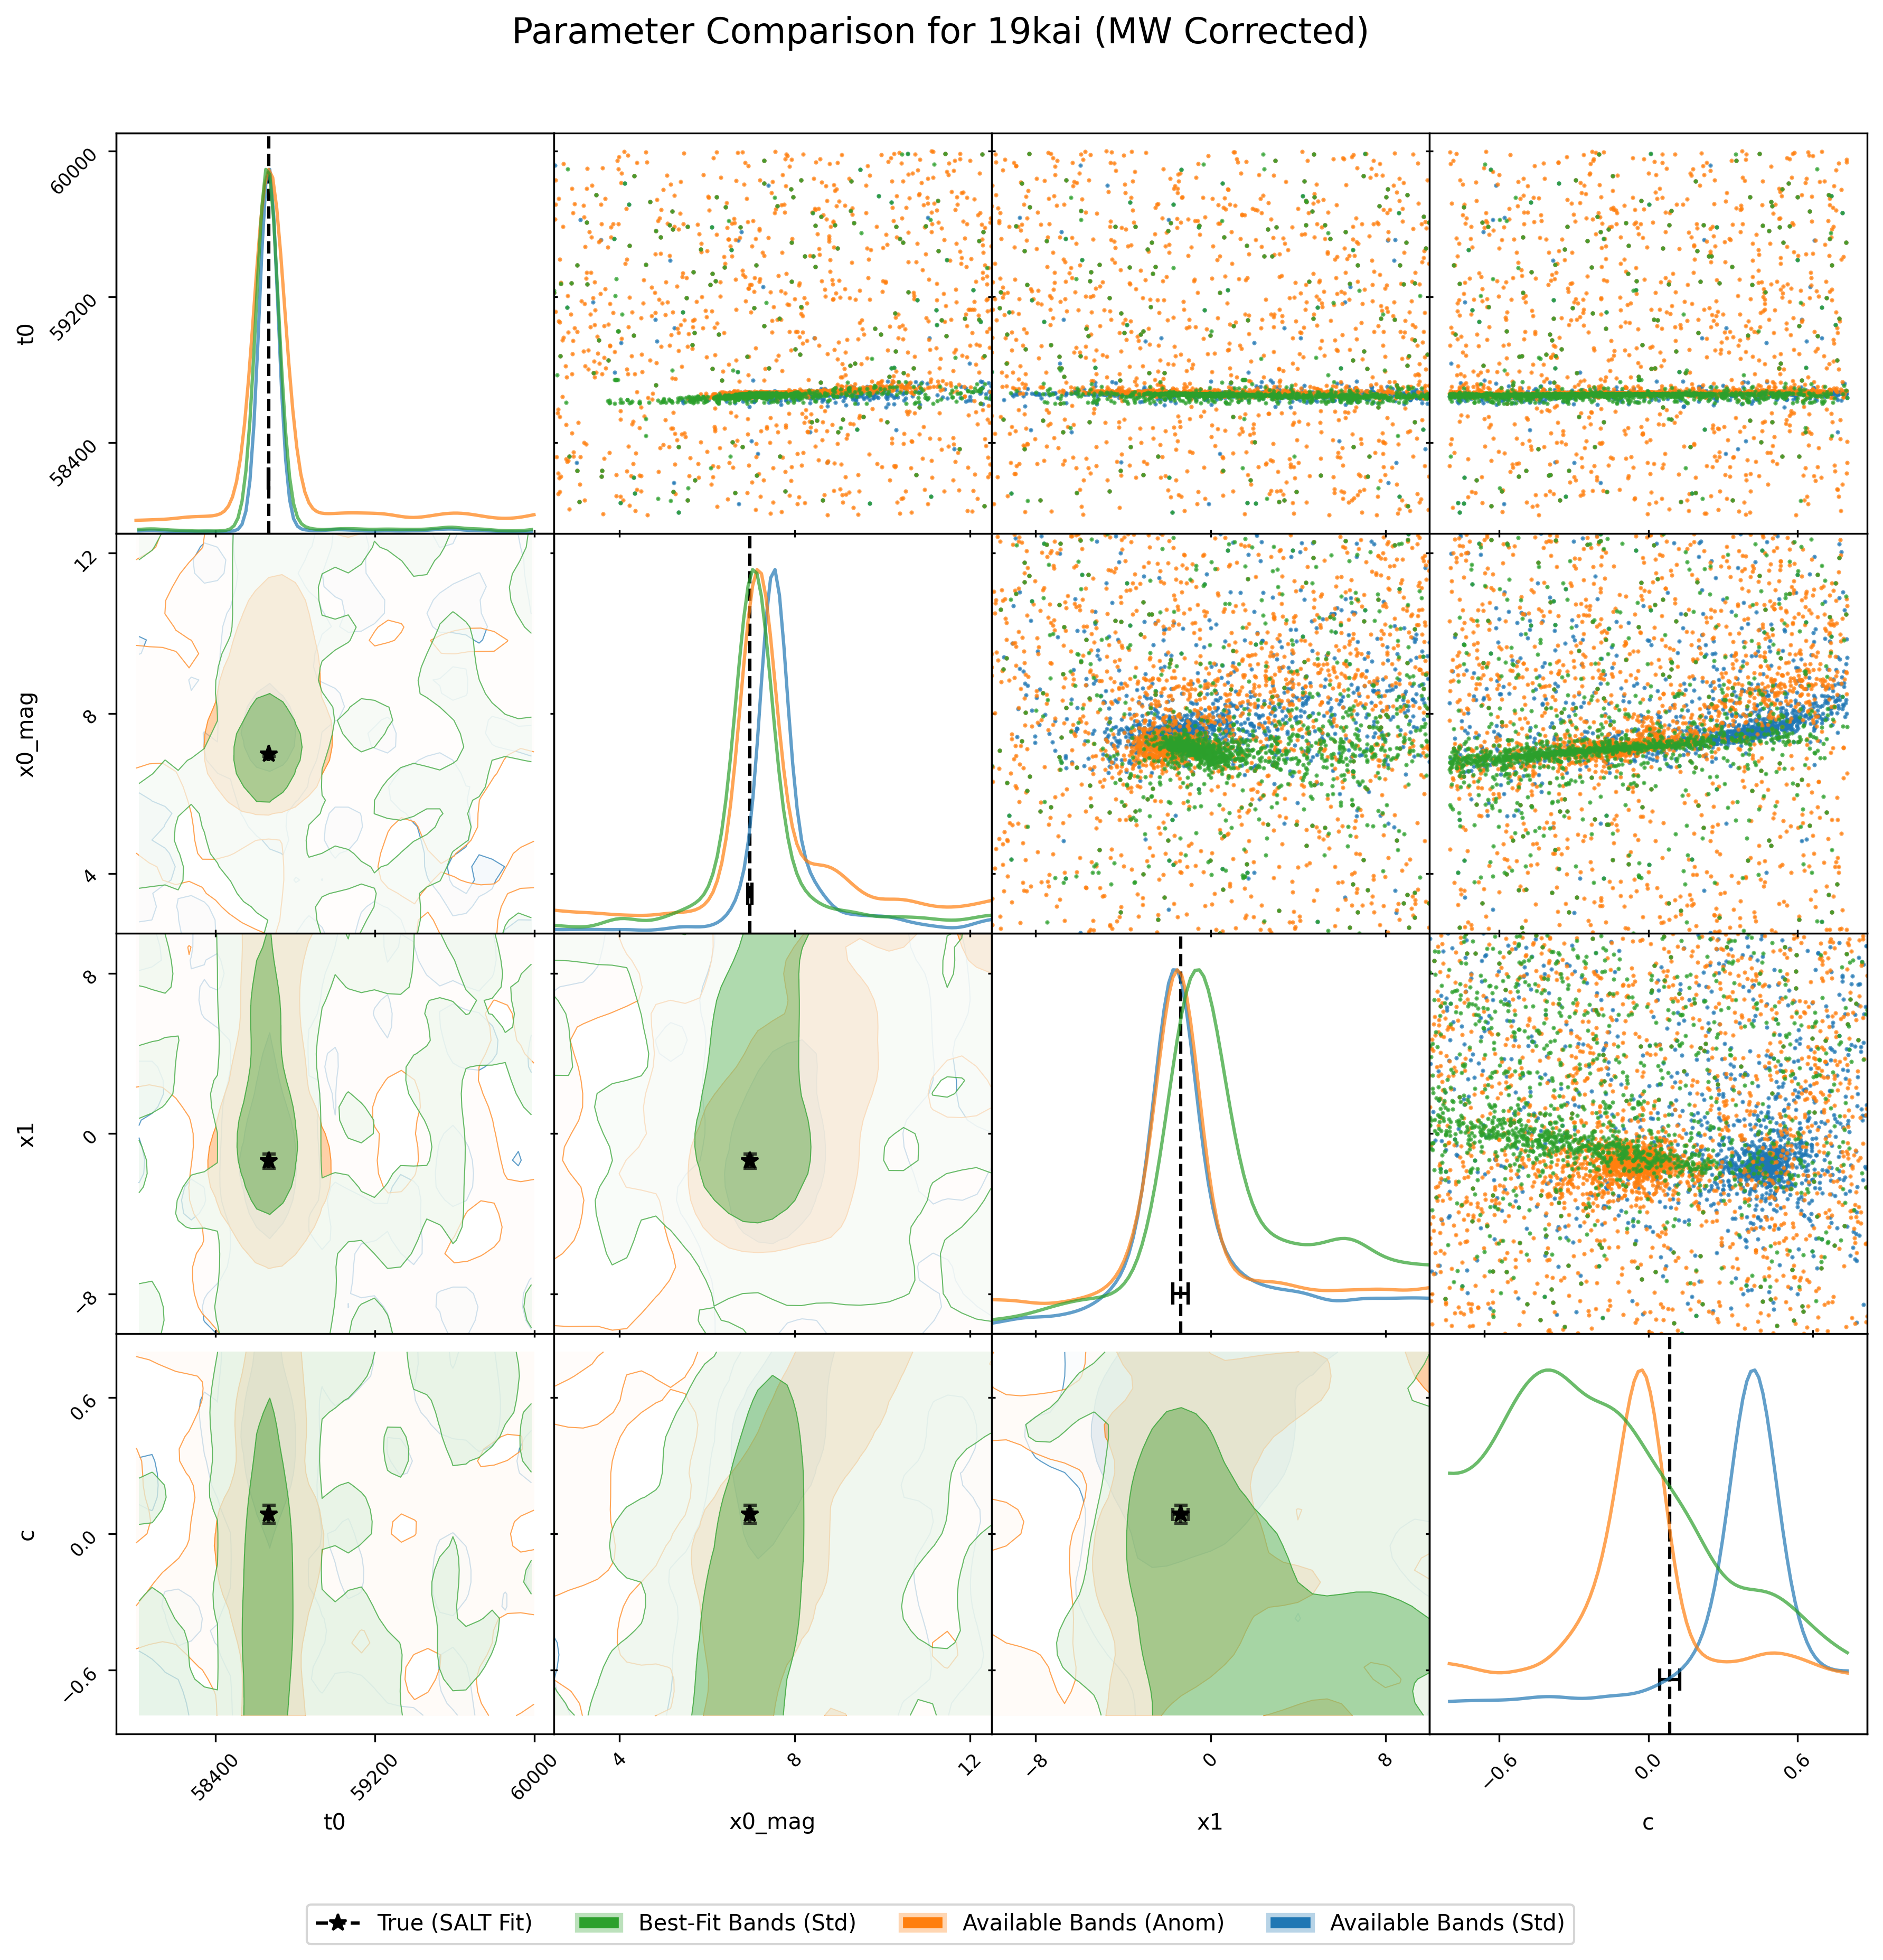
\includegraphics[width=1\textwidth]{images/corner_comparison_19kai.png}
  \end{columns}
\end{frame}


\begin{frame}{SN 20aczg: Light Curve and Corner Plot Comparison}
  \begin{columns}
    \column{0.5\textwidth}
    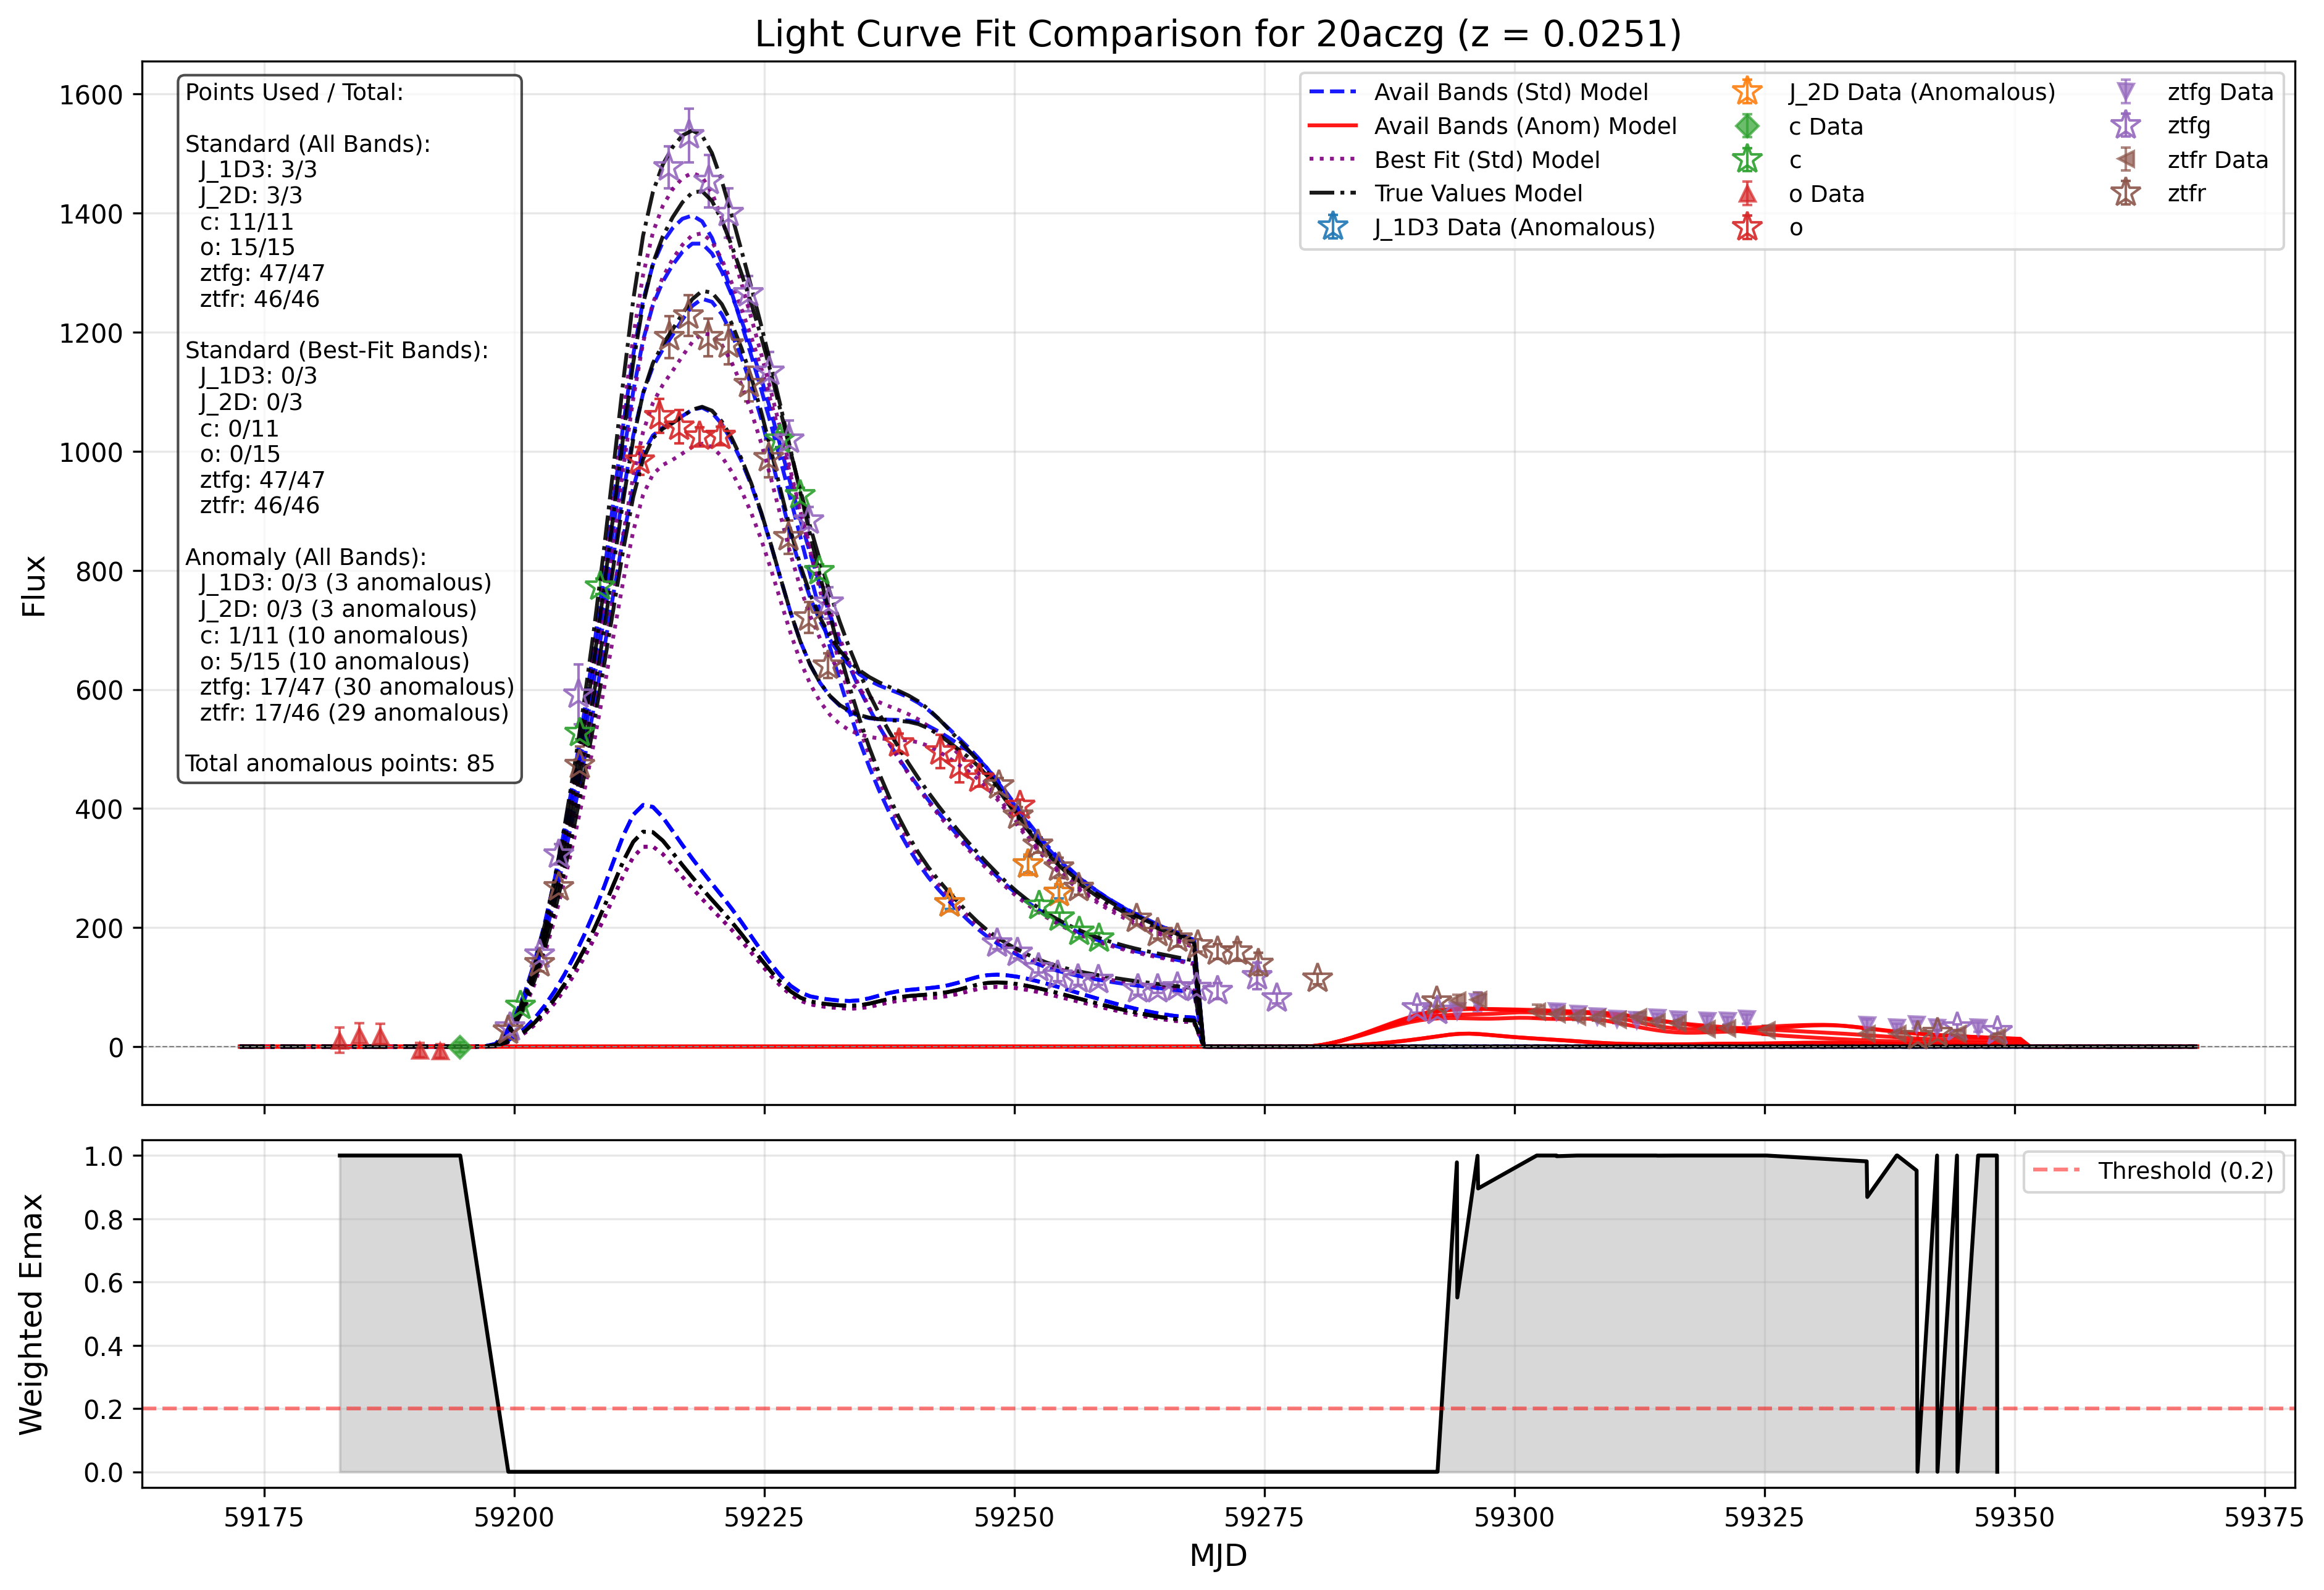
\includegraphics[width=1\textwidth]{images/light_curve_comparison_20aczg.png}
    \column{0.5\textwidth}
    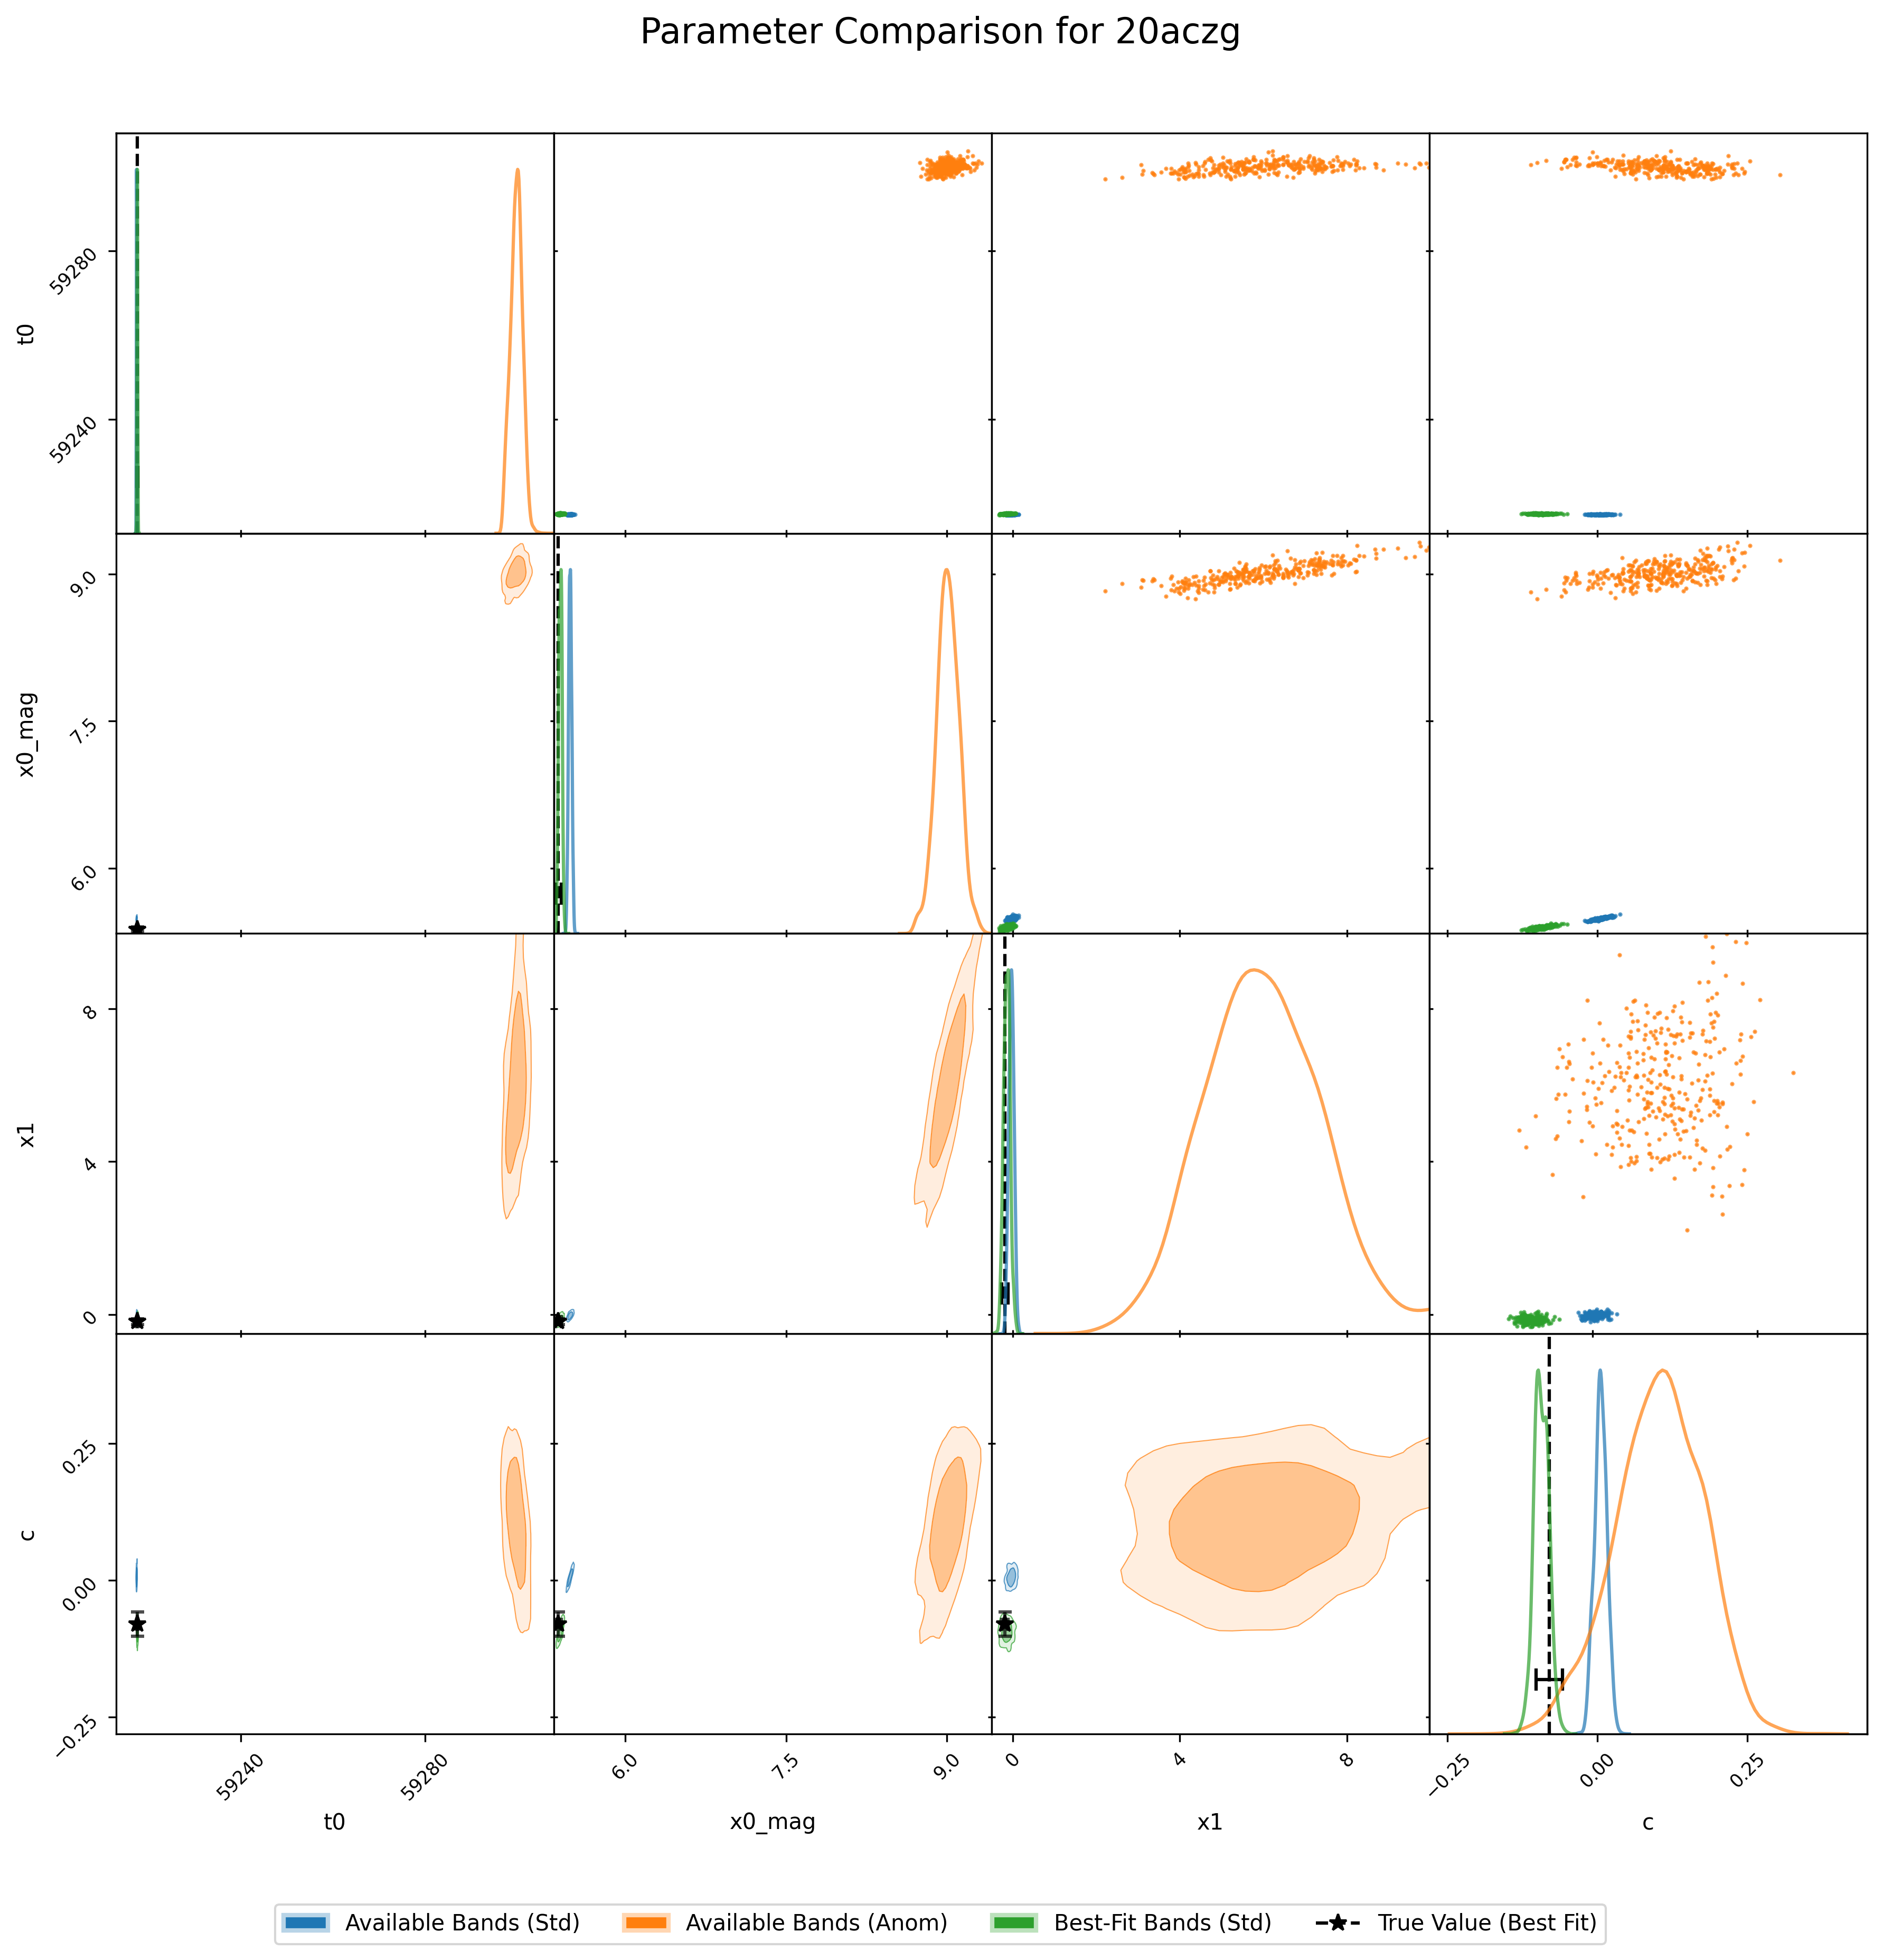
\includegraphics[width=1\textwidth]{images/corner_comparison_20aczg.png}
  \end{columns}
\end{frame}

\begin{frame}{Key points}
  \begin{enumerate}
    \item Standard flagging.
  \end{enumerate}
\end{frame}

\begin{frame}{Key points}
  \begin{enumerate}
    \item Standard flagging.
    \item Automated filter selection.
  \end{enumerate}
\end{frame}

\begin{frame}{Key points}
  \begin{enumerate}
    \item Standard flagging.
    \item Automated filter selection.
    \item Data preservation from previously discarded filters.
    \item Potentially can flag non Ia automatically?
  \end{enumerate}
\end{frame}

\begin{frame}{Next steps}
  \begin{itemize}
    \item Assess Hubble diagrams 
      \begin{itemize}
        \item Quantify impact on cosmological parameter estimation
        \item Compare with traditional outlier rejection methods
        \item Evaluate systematic error reduction
      \end{itemize}
    \item Try on other datasets?
      \begin{itemize}
        \item Apply to different supernova surveys (ZTF, LSST)
        \item Test with different photometric systems
        \item Evaluate performance across redshift ranges
      \end{itemize}
  \end{itemize}
\end{frame}

\section{What next}

\begin{frame}{What do(nt) we look for?}
  \begin{columns}
    \column{0.5\textwidth}
      \centering
      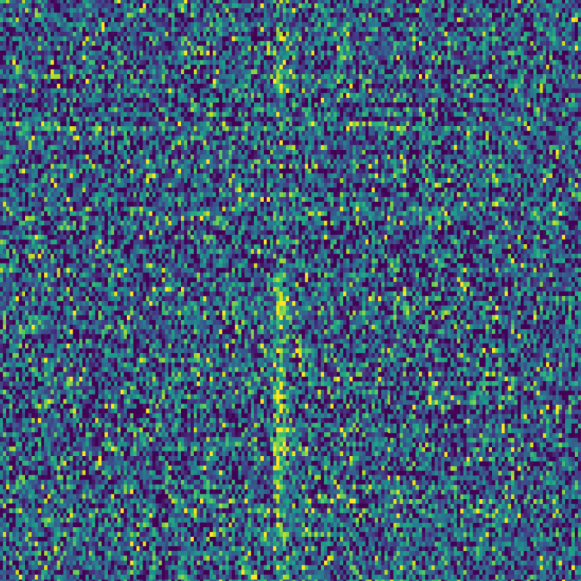
\includegraphics[width=0.9\textwidth]{images/frb.png}
    \column{0.5\textwidth}
      \begin{itemize}
        \item New science often found when looking for something else.
        \item How to search for something unknown?
        \item How much new science was missed in old data?
      \end{itemize}
  \end{columns}
\end{frame}

\end{document}